
\chapter{Projektowanie interfejsu użytkownika dla systemu FastPost Express}

\section{Założenia projektowe i strategia UI/UX}
Projekt interfejsu systemu \textbf{FastPost Express} został opracowany z myślą o maksymalizacji efektywności procesów logistycznych przy jednoczesnym zachowaniu niskiego progu wejścia dla użytkownika końcowego. Architektura informacji opiera się na metodologii \textit{User-Centered Design}, koncentrując się na następujących filarach:

\begin{itemize}
    \item \textbf{Intuicyjność:} Wykorzystanie powszechnie znanych wzorców projektowych (Design Patterns), co skraca czas adaptacji użytkownika.
    \item \textbf{Responsywność:} Adaptacja układu graficznego do różnych rozdzielczości ekranowych, zapewniająca komfort pracy zarówno kurierom w terenie, jak i administratorom w biurze.
    \textbf{Hierarchia wizualna:} Zastosowanie kontrastu i typografii do separacji danych krytycznych od informacji pomocniczych.
\end{itemize}

\section{System autentykacji i onboarding}
Proces dostępu do systemu został zaprojektowany w sposób liniowy, minimalizując liczbę kroków niezbędnych do rozpoczęcia pracy. Zastosowano mechanizmy zwiększające bezpieczeństwo oraz jakość wprowadzanych danych:

\begin{itemize}
    \item \textbf{Walidacja \textit{inline}:} Informowanie o błędach w formatowaniu (np. błędny format e-mail) w czasie rzeczywistym.
    \item \textbf{Weryfikacja tożsamości:} Dwuetapowy proces weryfikacji konta.
\end{itemize}

\section{Proces autentykacji i rejestracji}
Zgodnie ze sprawdzonymi wzorcami projektowymi, proces wprowadzania danych wykorzystuje placeholdery oraz walidację w czasie rzeczywistym. Po rejestracji użytkownik przechodzi proces weryfikacji tożsamości.

\begin{figure}[H]
    \centering
    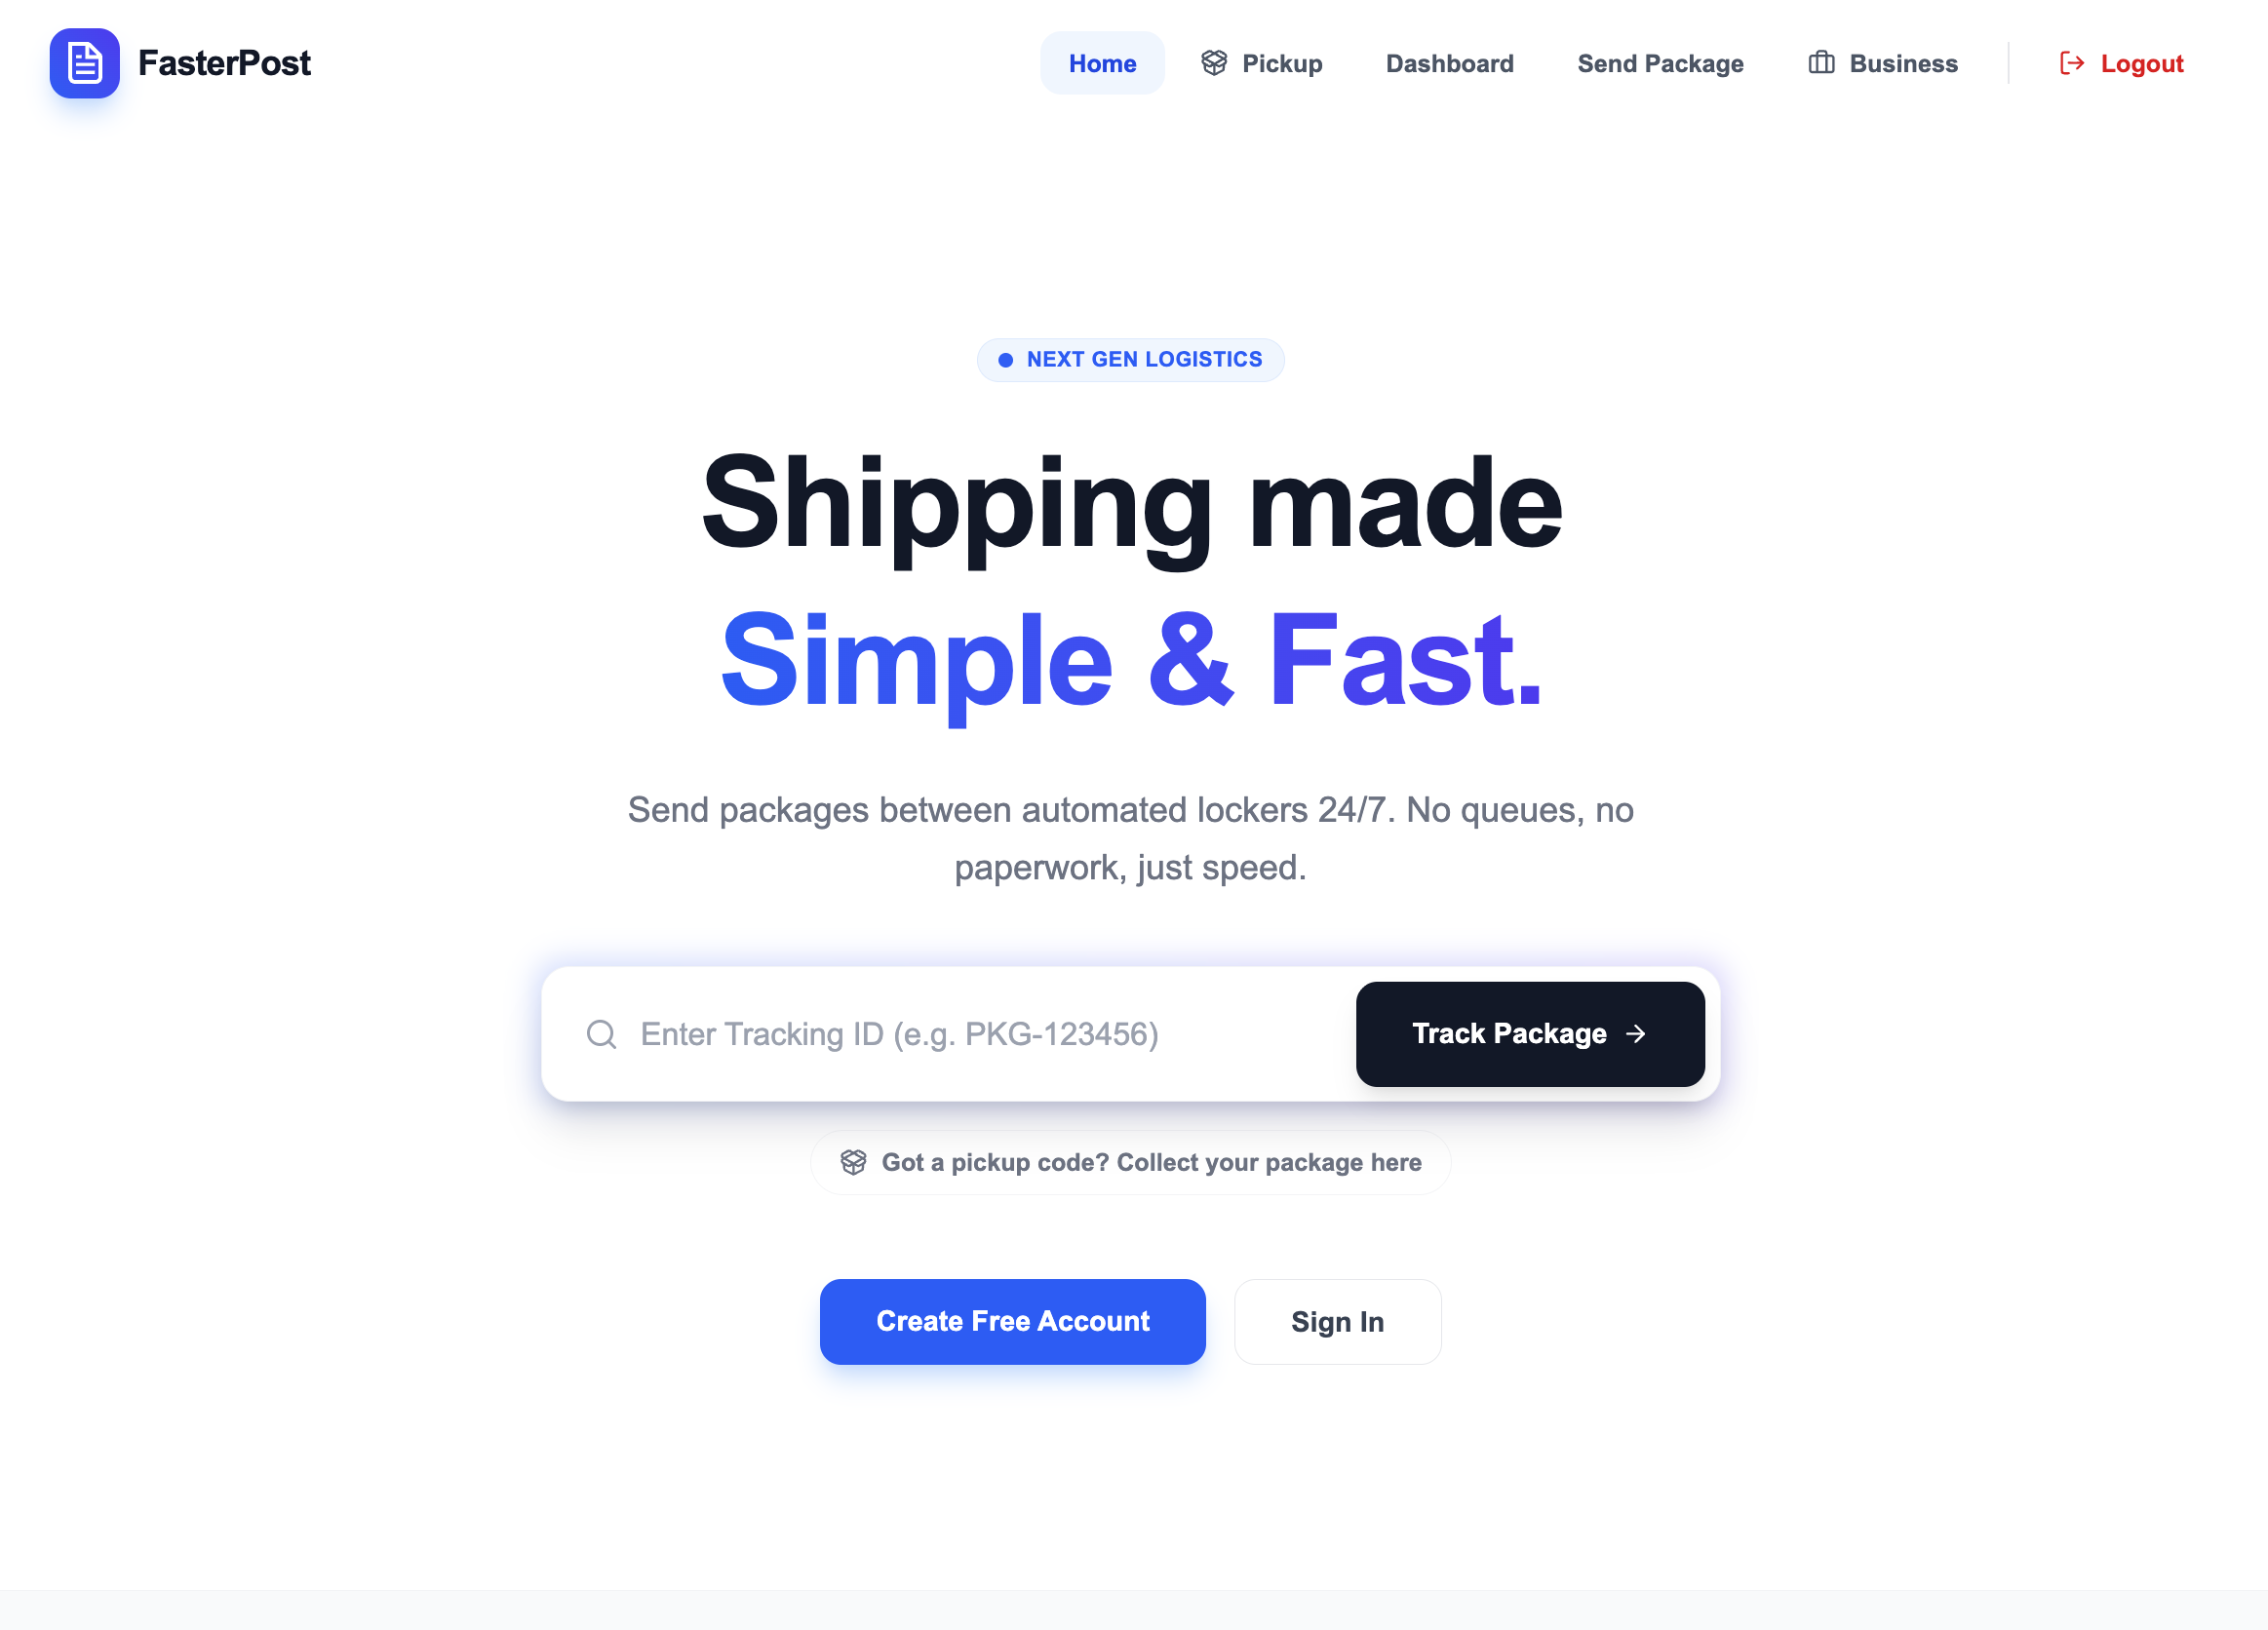
\includegraphics[width=0.5\textwidth]{../screenshots/1_home_page.png}
    \caption{Strona główna z nawigacją górną (Top Navigation).}
\end{figure}

\begin{figure}[H]
    \centering
    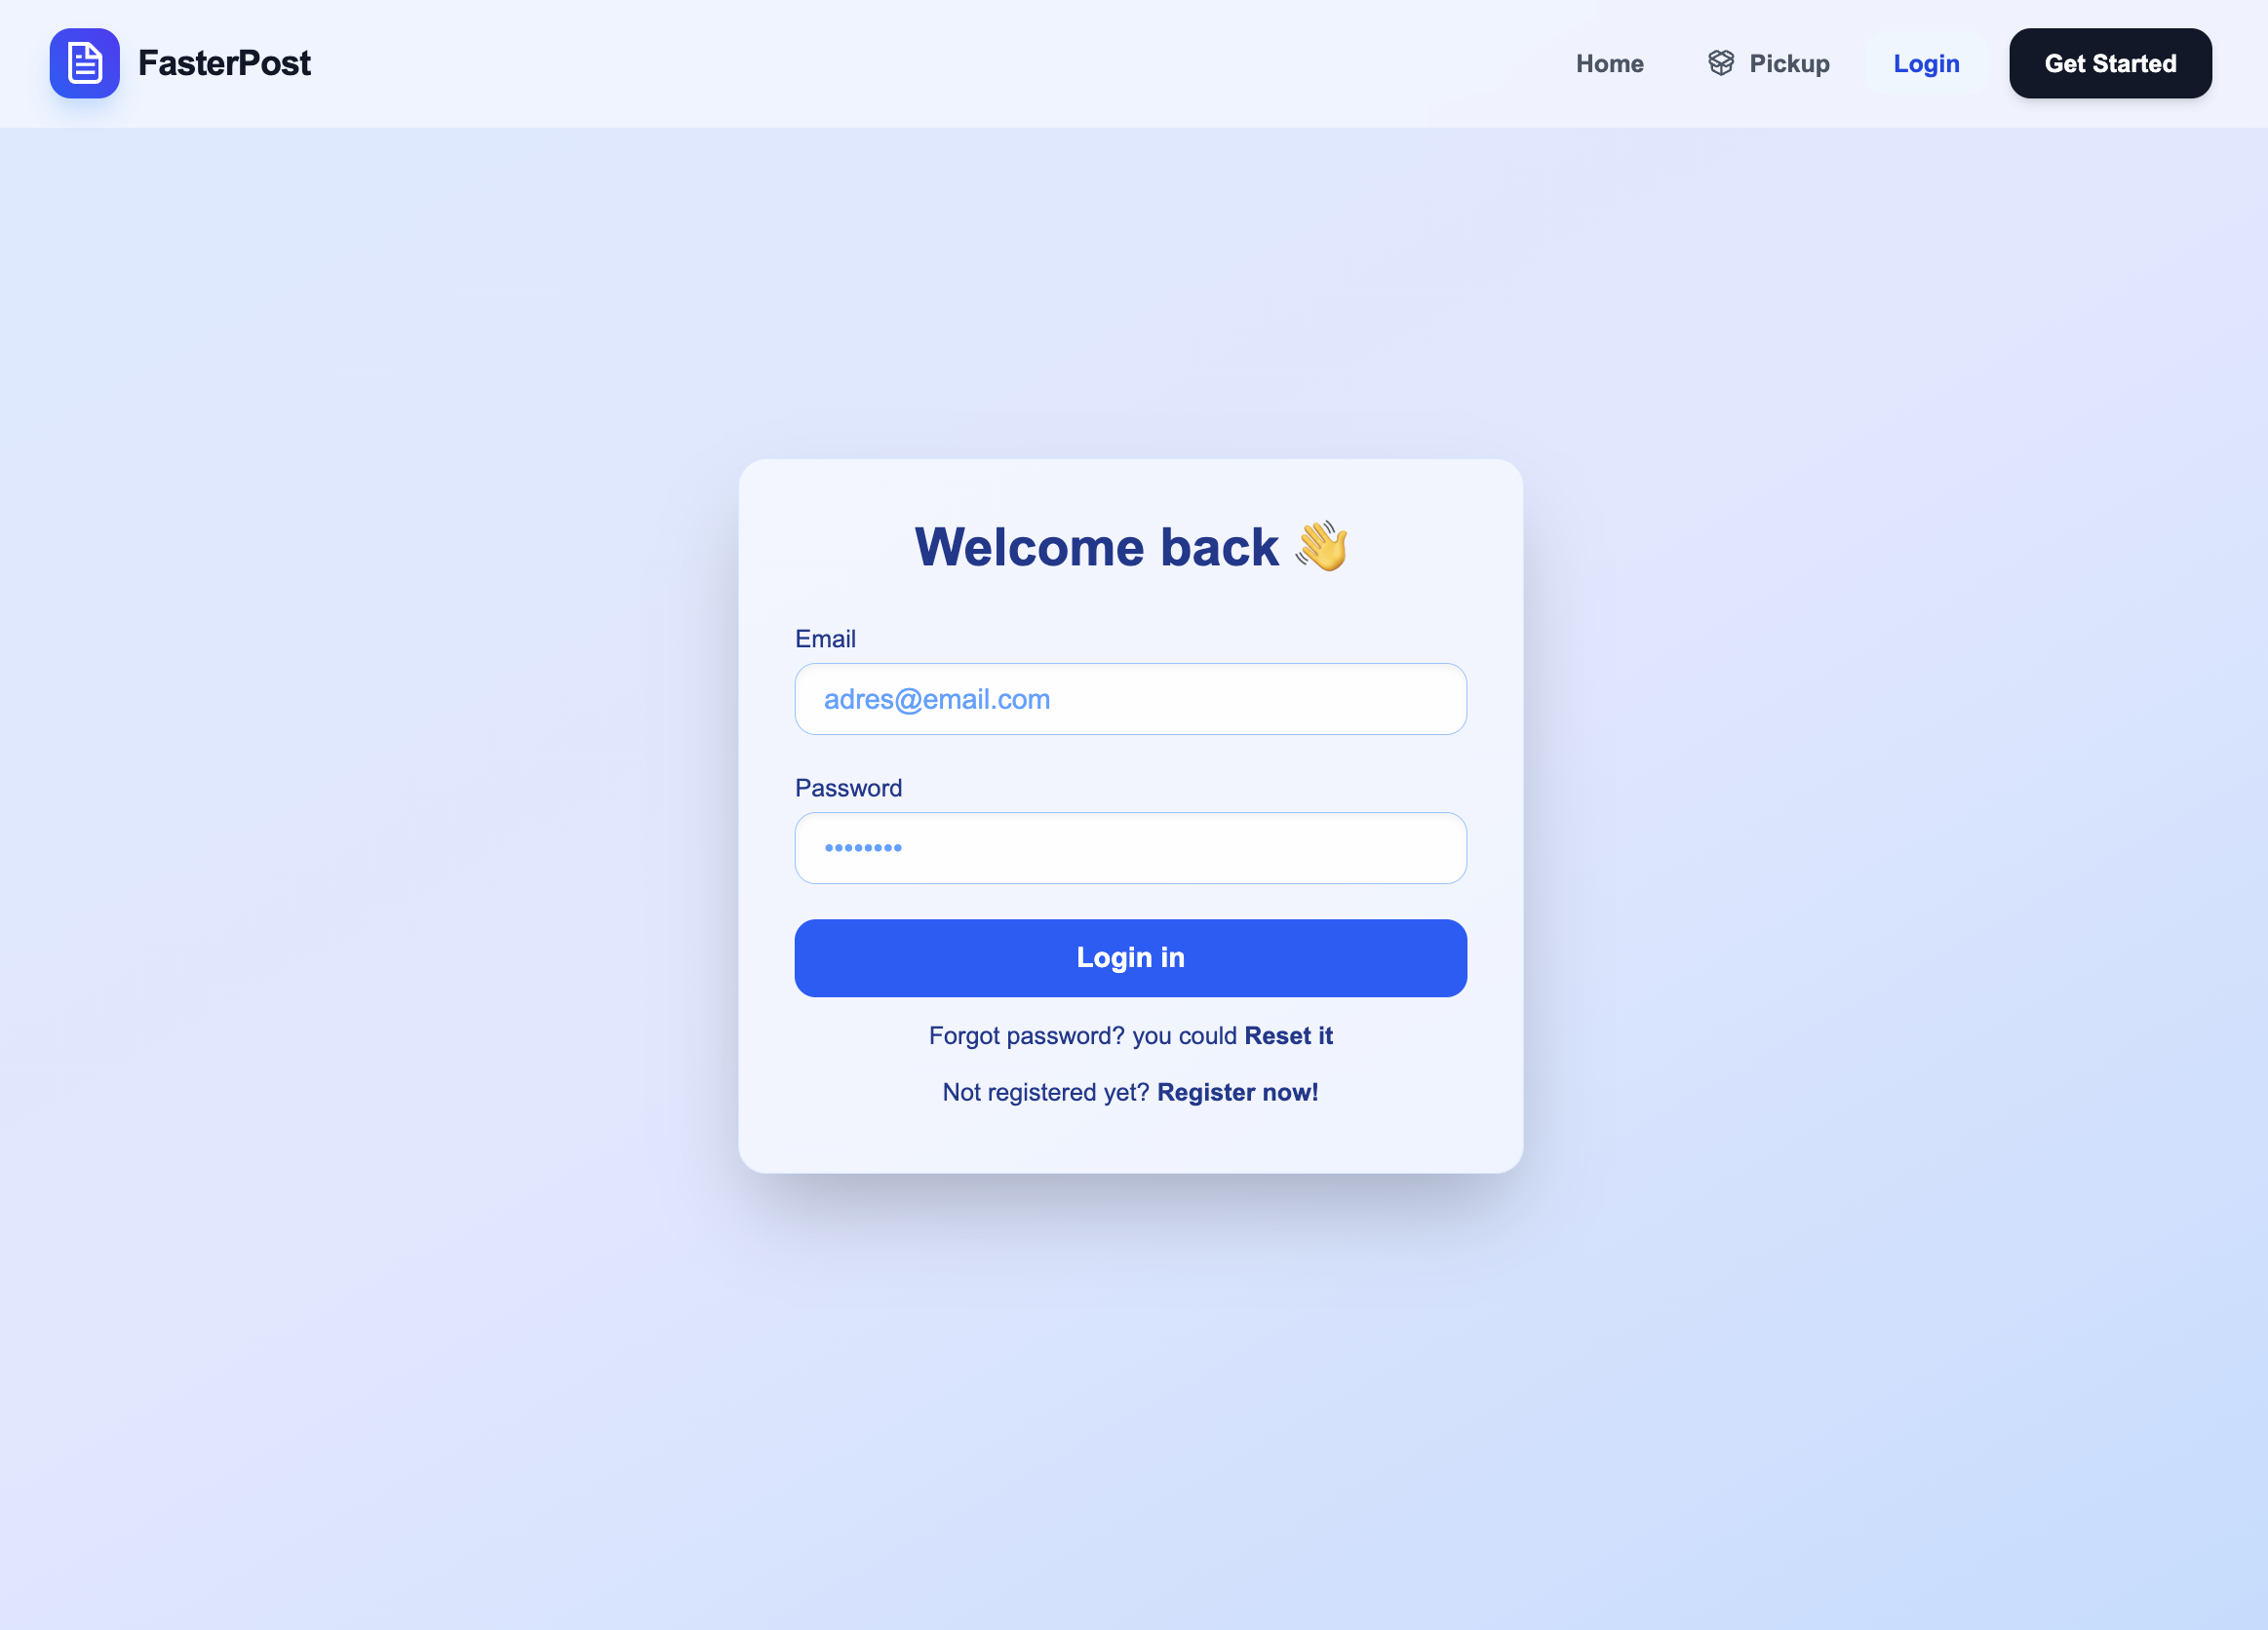
\includegraphics[width=0.45\textwidth]{../screenshots/2_login_screen.png}
    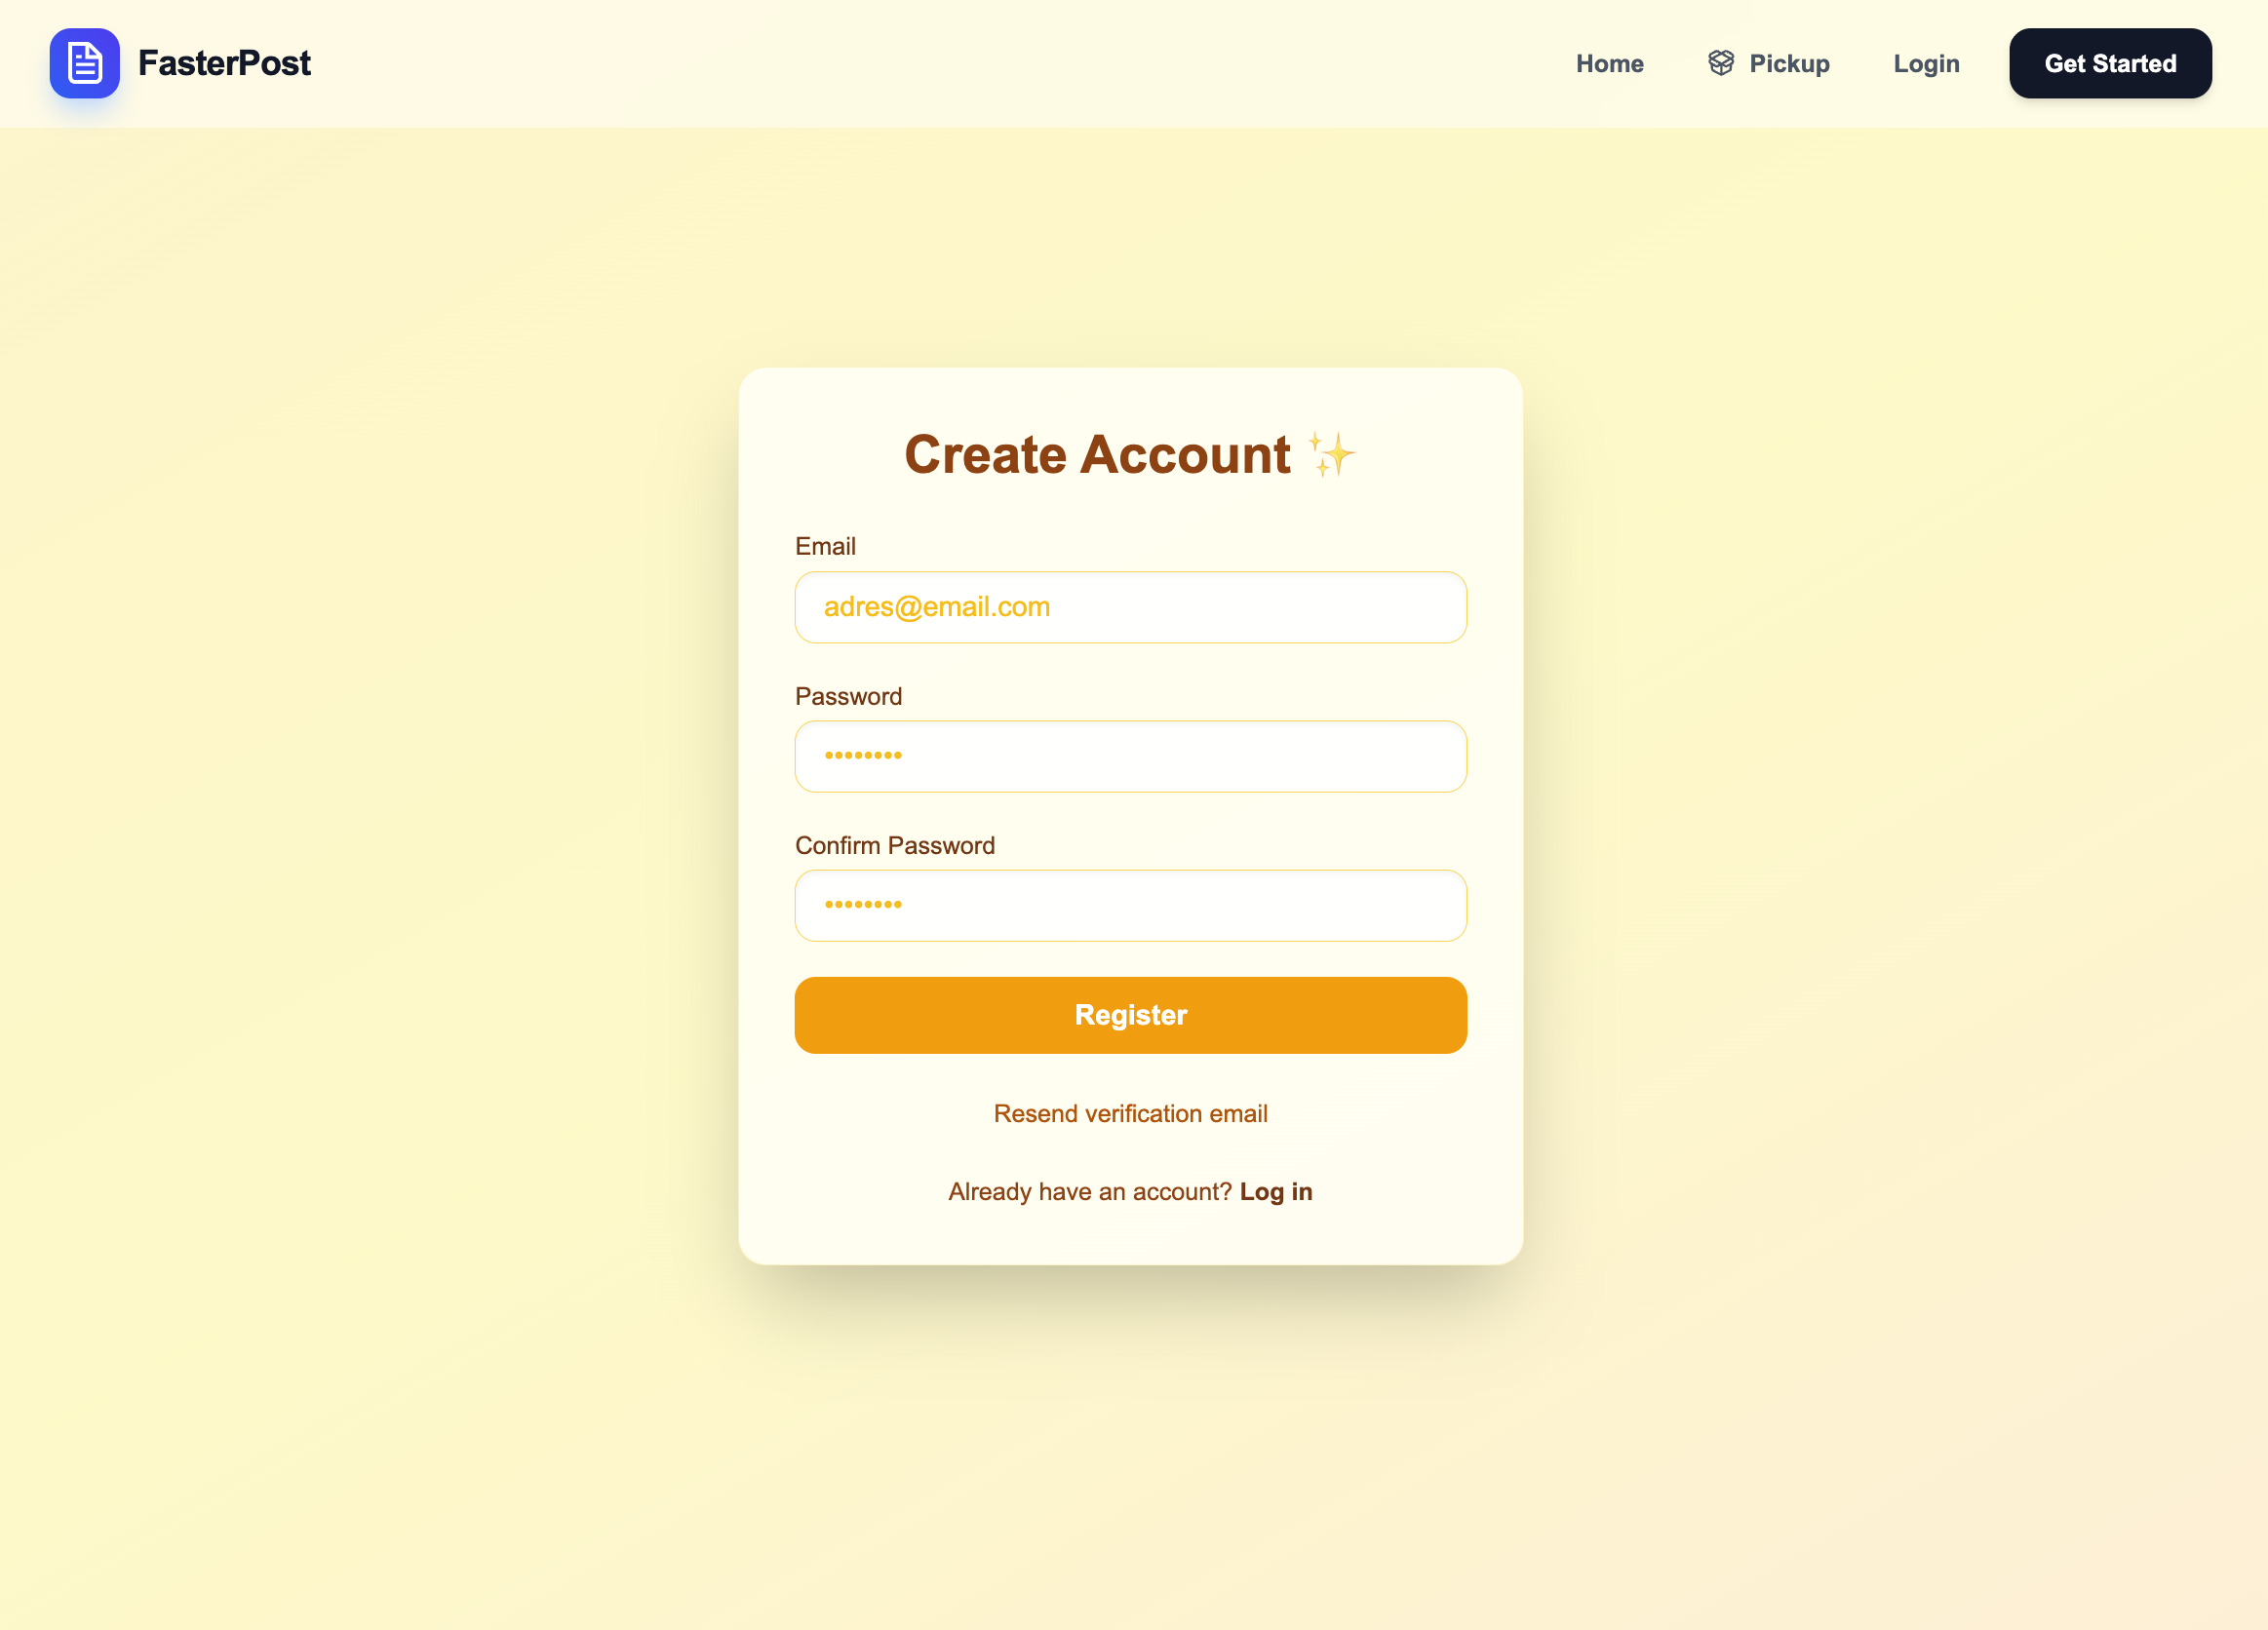
\includegraphics[width=0.45\textwidth]{../screenshots/3_register_screen.png}
    \caption{Ekran logowania i rejestracji z polami tekstowymi.}
\end{figure}

\begin{figure}[H]
    \centering
    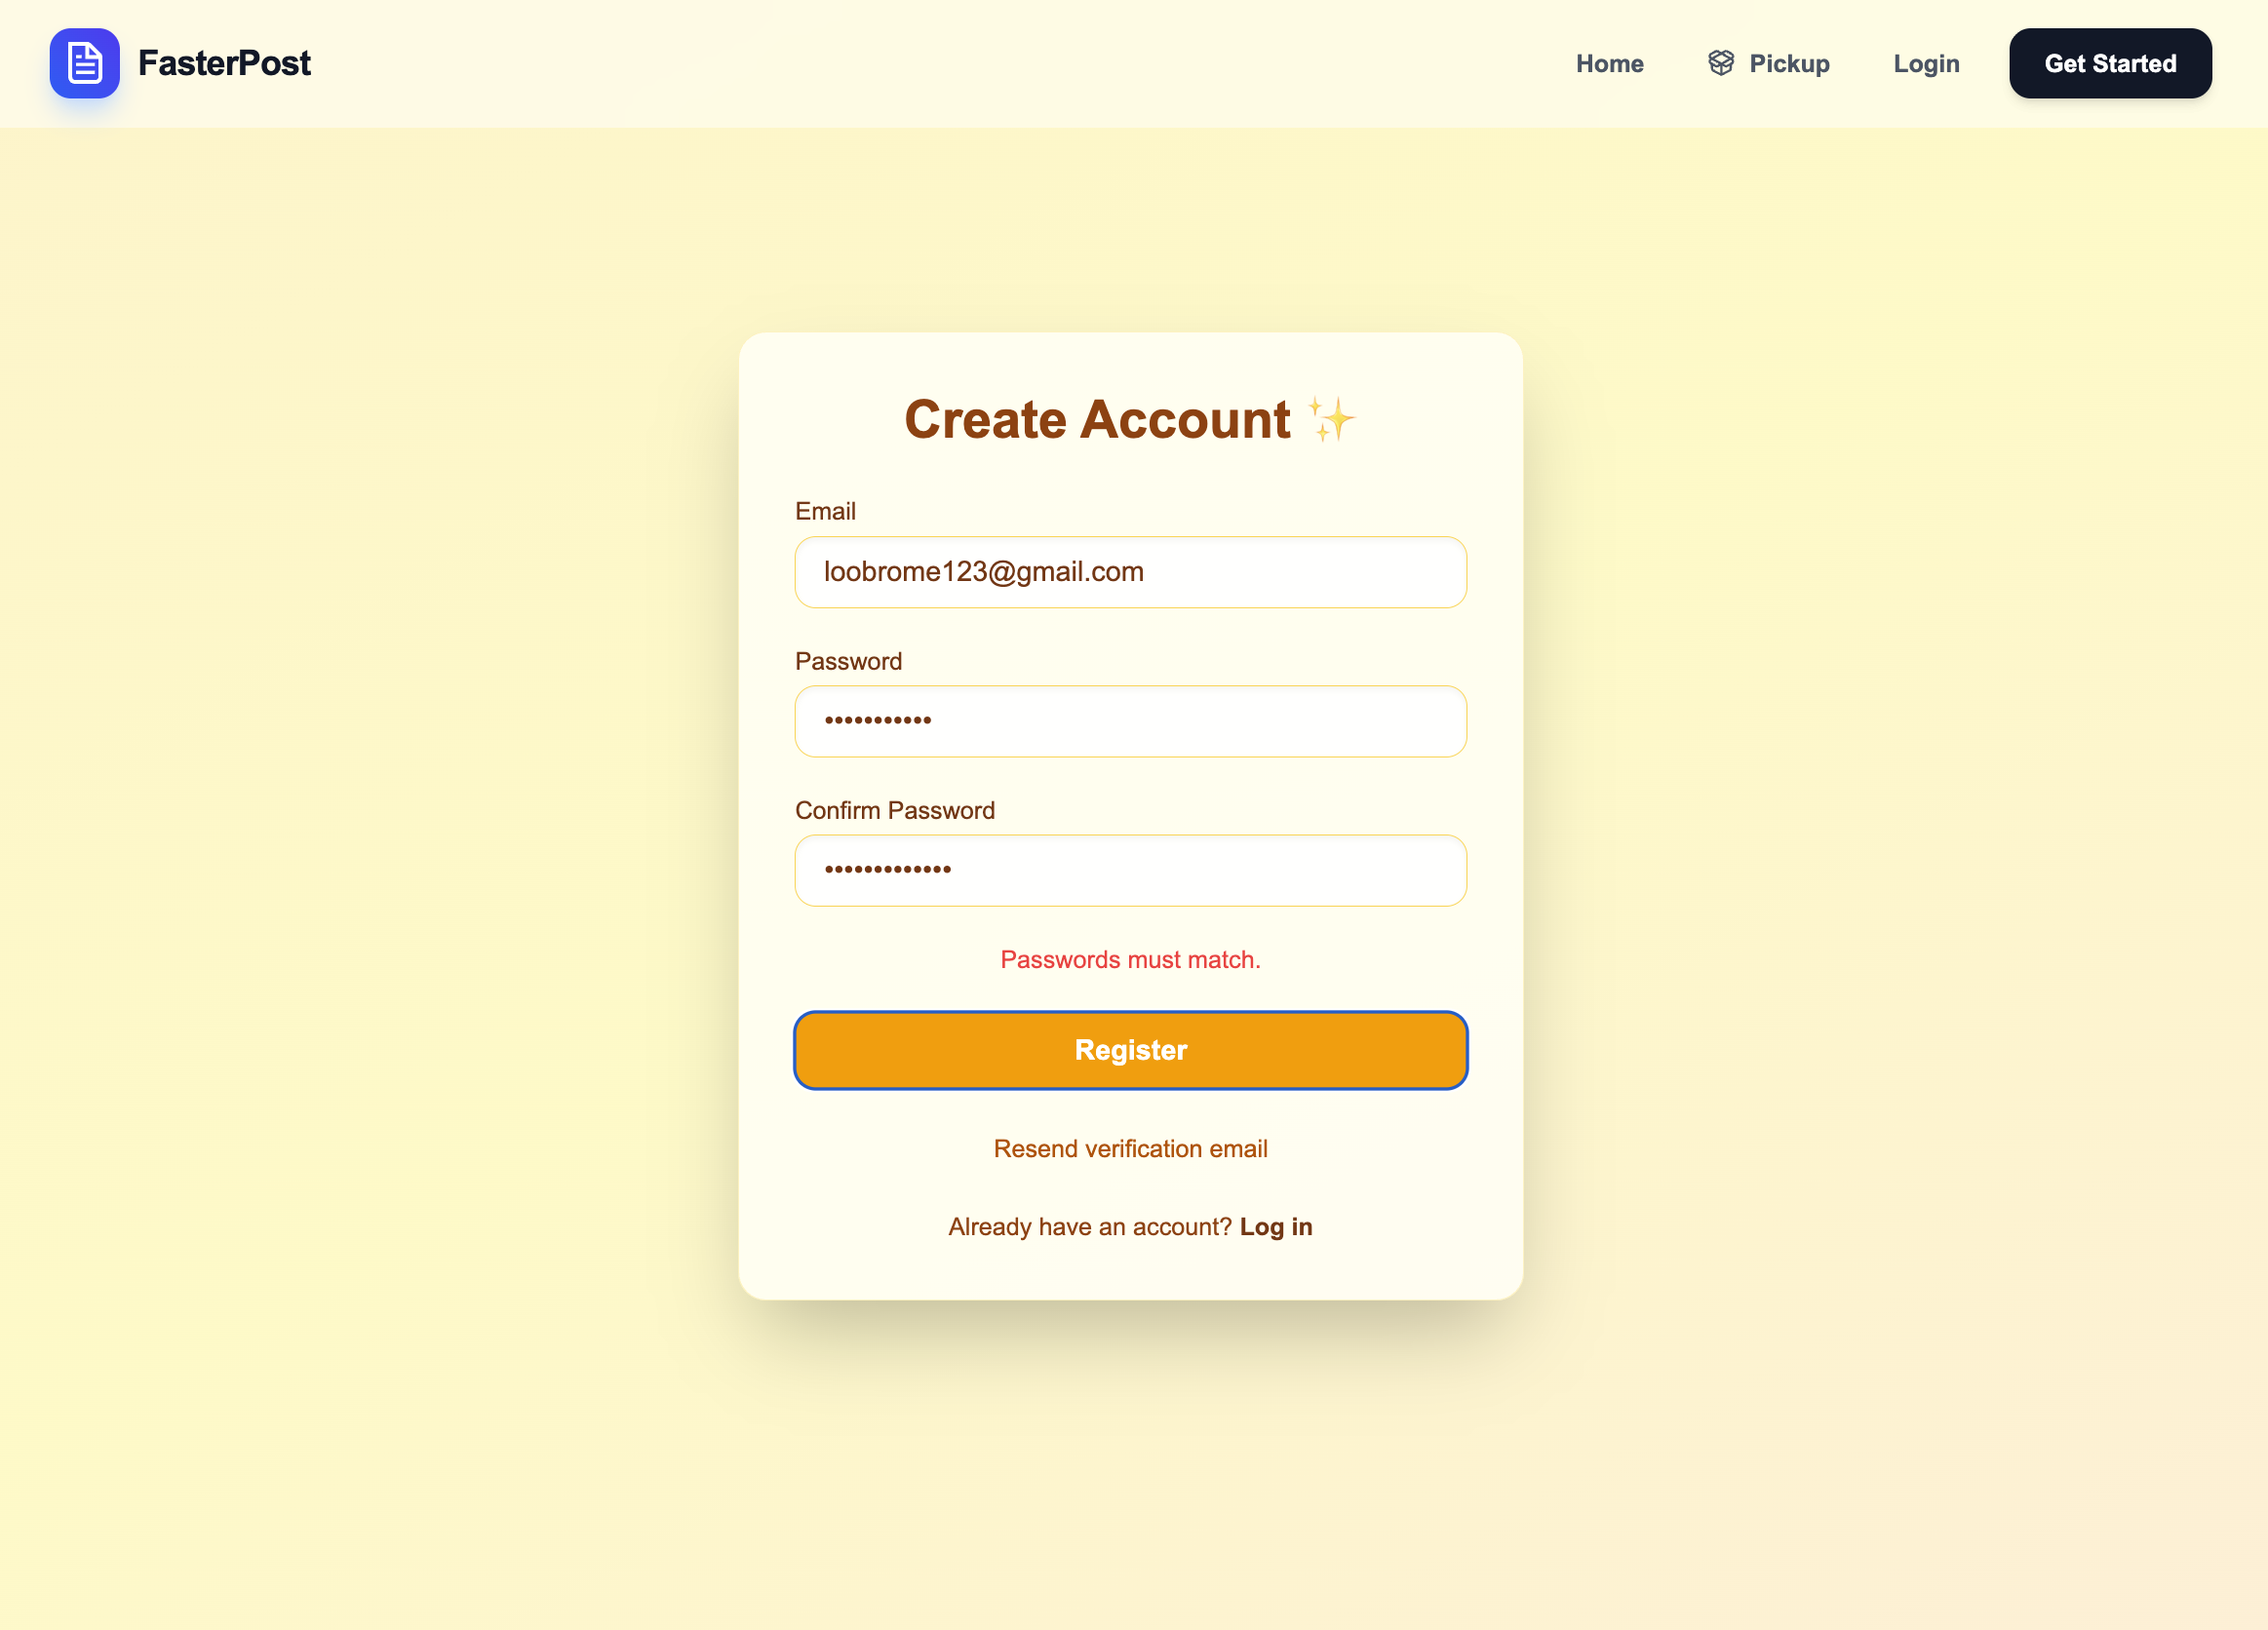
\includegraphics[width=0.45\textwidth]{../screenshots/3_register_screen_invalid_input.png}
    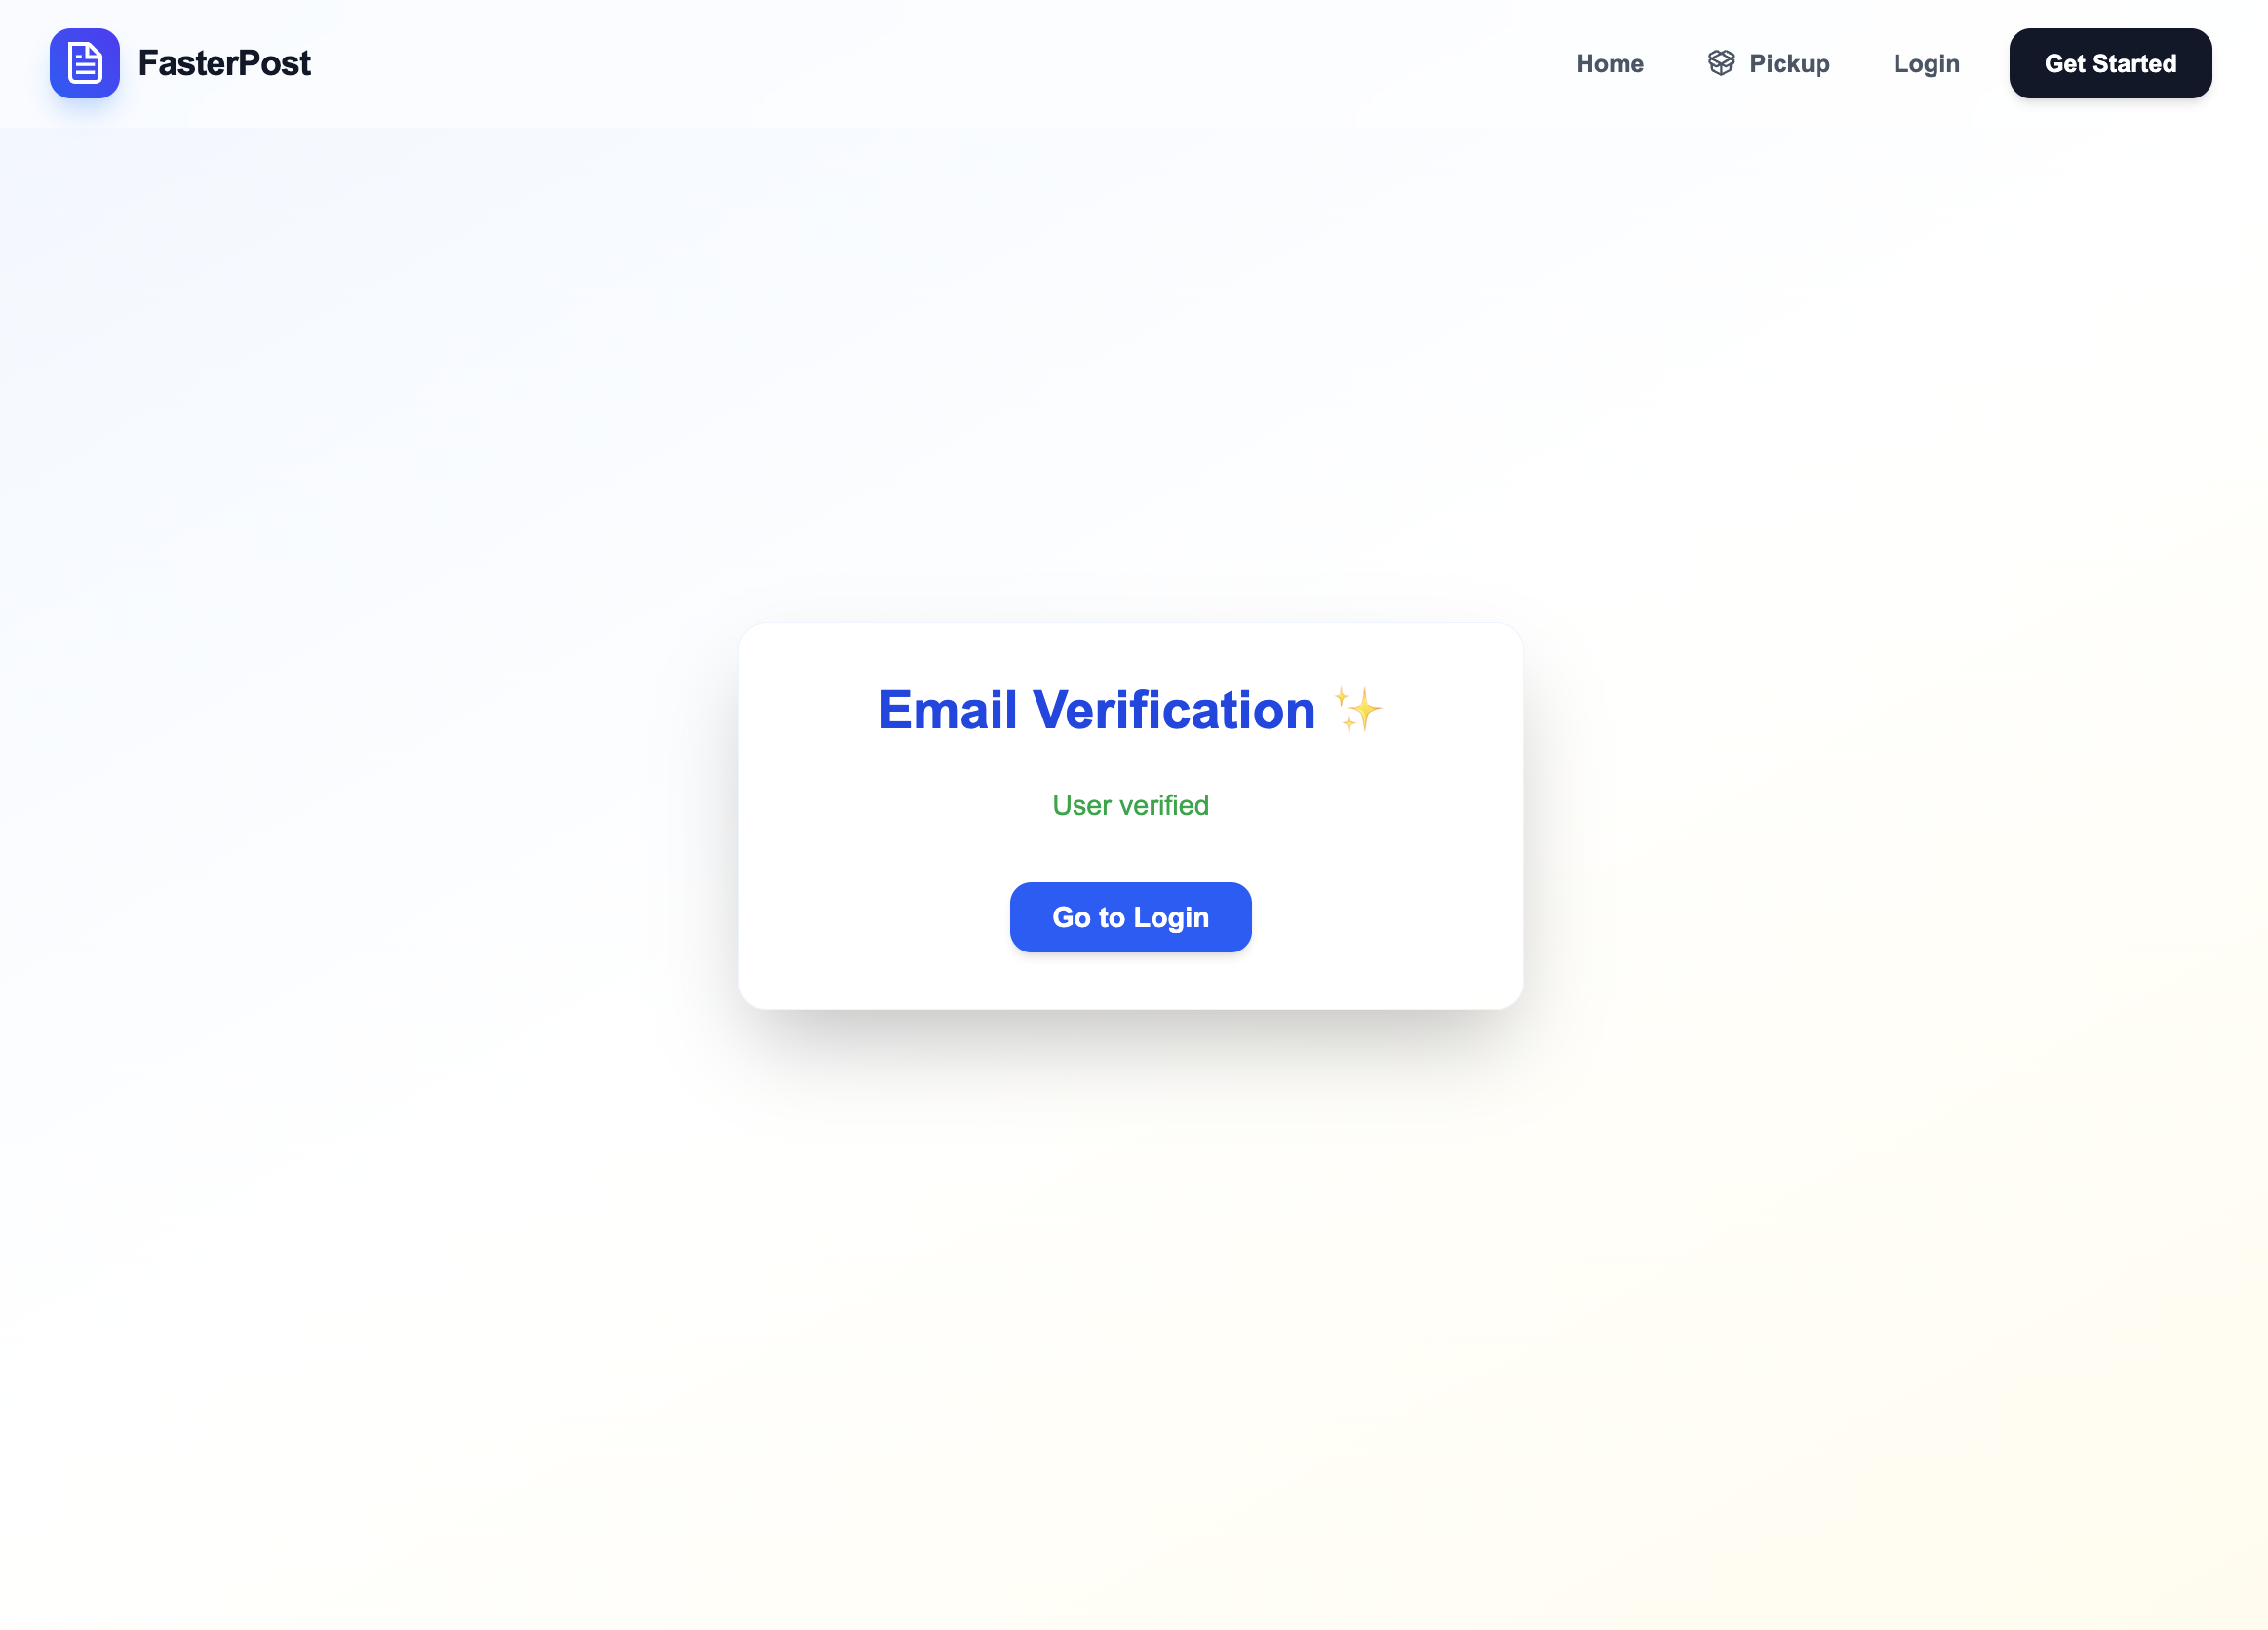
\includegraphics[width=0.45\textwidth]{../screenshots/4_email_verification.png}
    \caption{Walidacja błędów w czasie rzeczywistym oraz ekran weryfikacji adresu e-mail.}
\end{figure}

\section{Panele użytkownika i funkcjonalności}
Interfejs wykorzystuje karty (Cards) do przeglądania treści oraz paski postępu do informowania o stanie operacji.

\subsection{Pulpit i obsługa przesyłek - użytkownik indywidualny}
Użytkownik ma możliwość zarządzania swoimi paczkami, opłacania ich oraz śledzenia statusu w czasie rzeczywistym.

\begin{figure}[H]
    \centering
    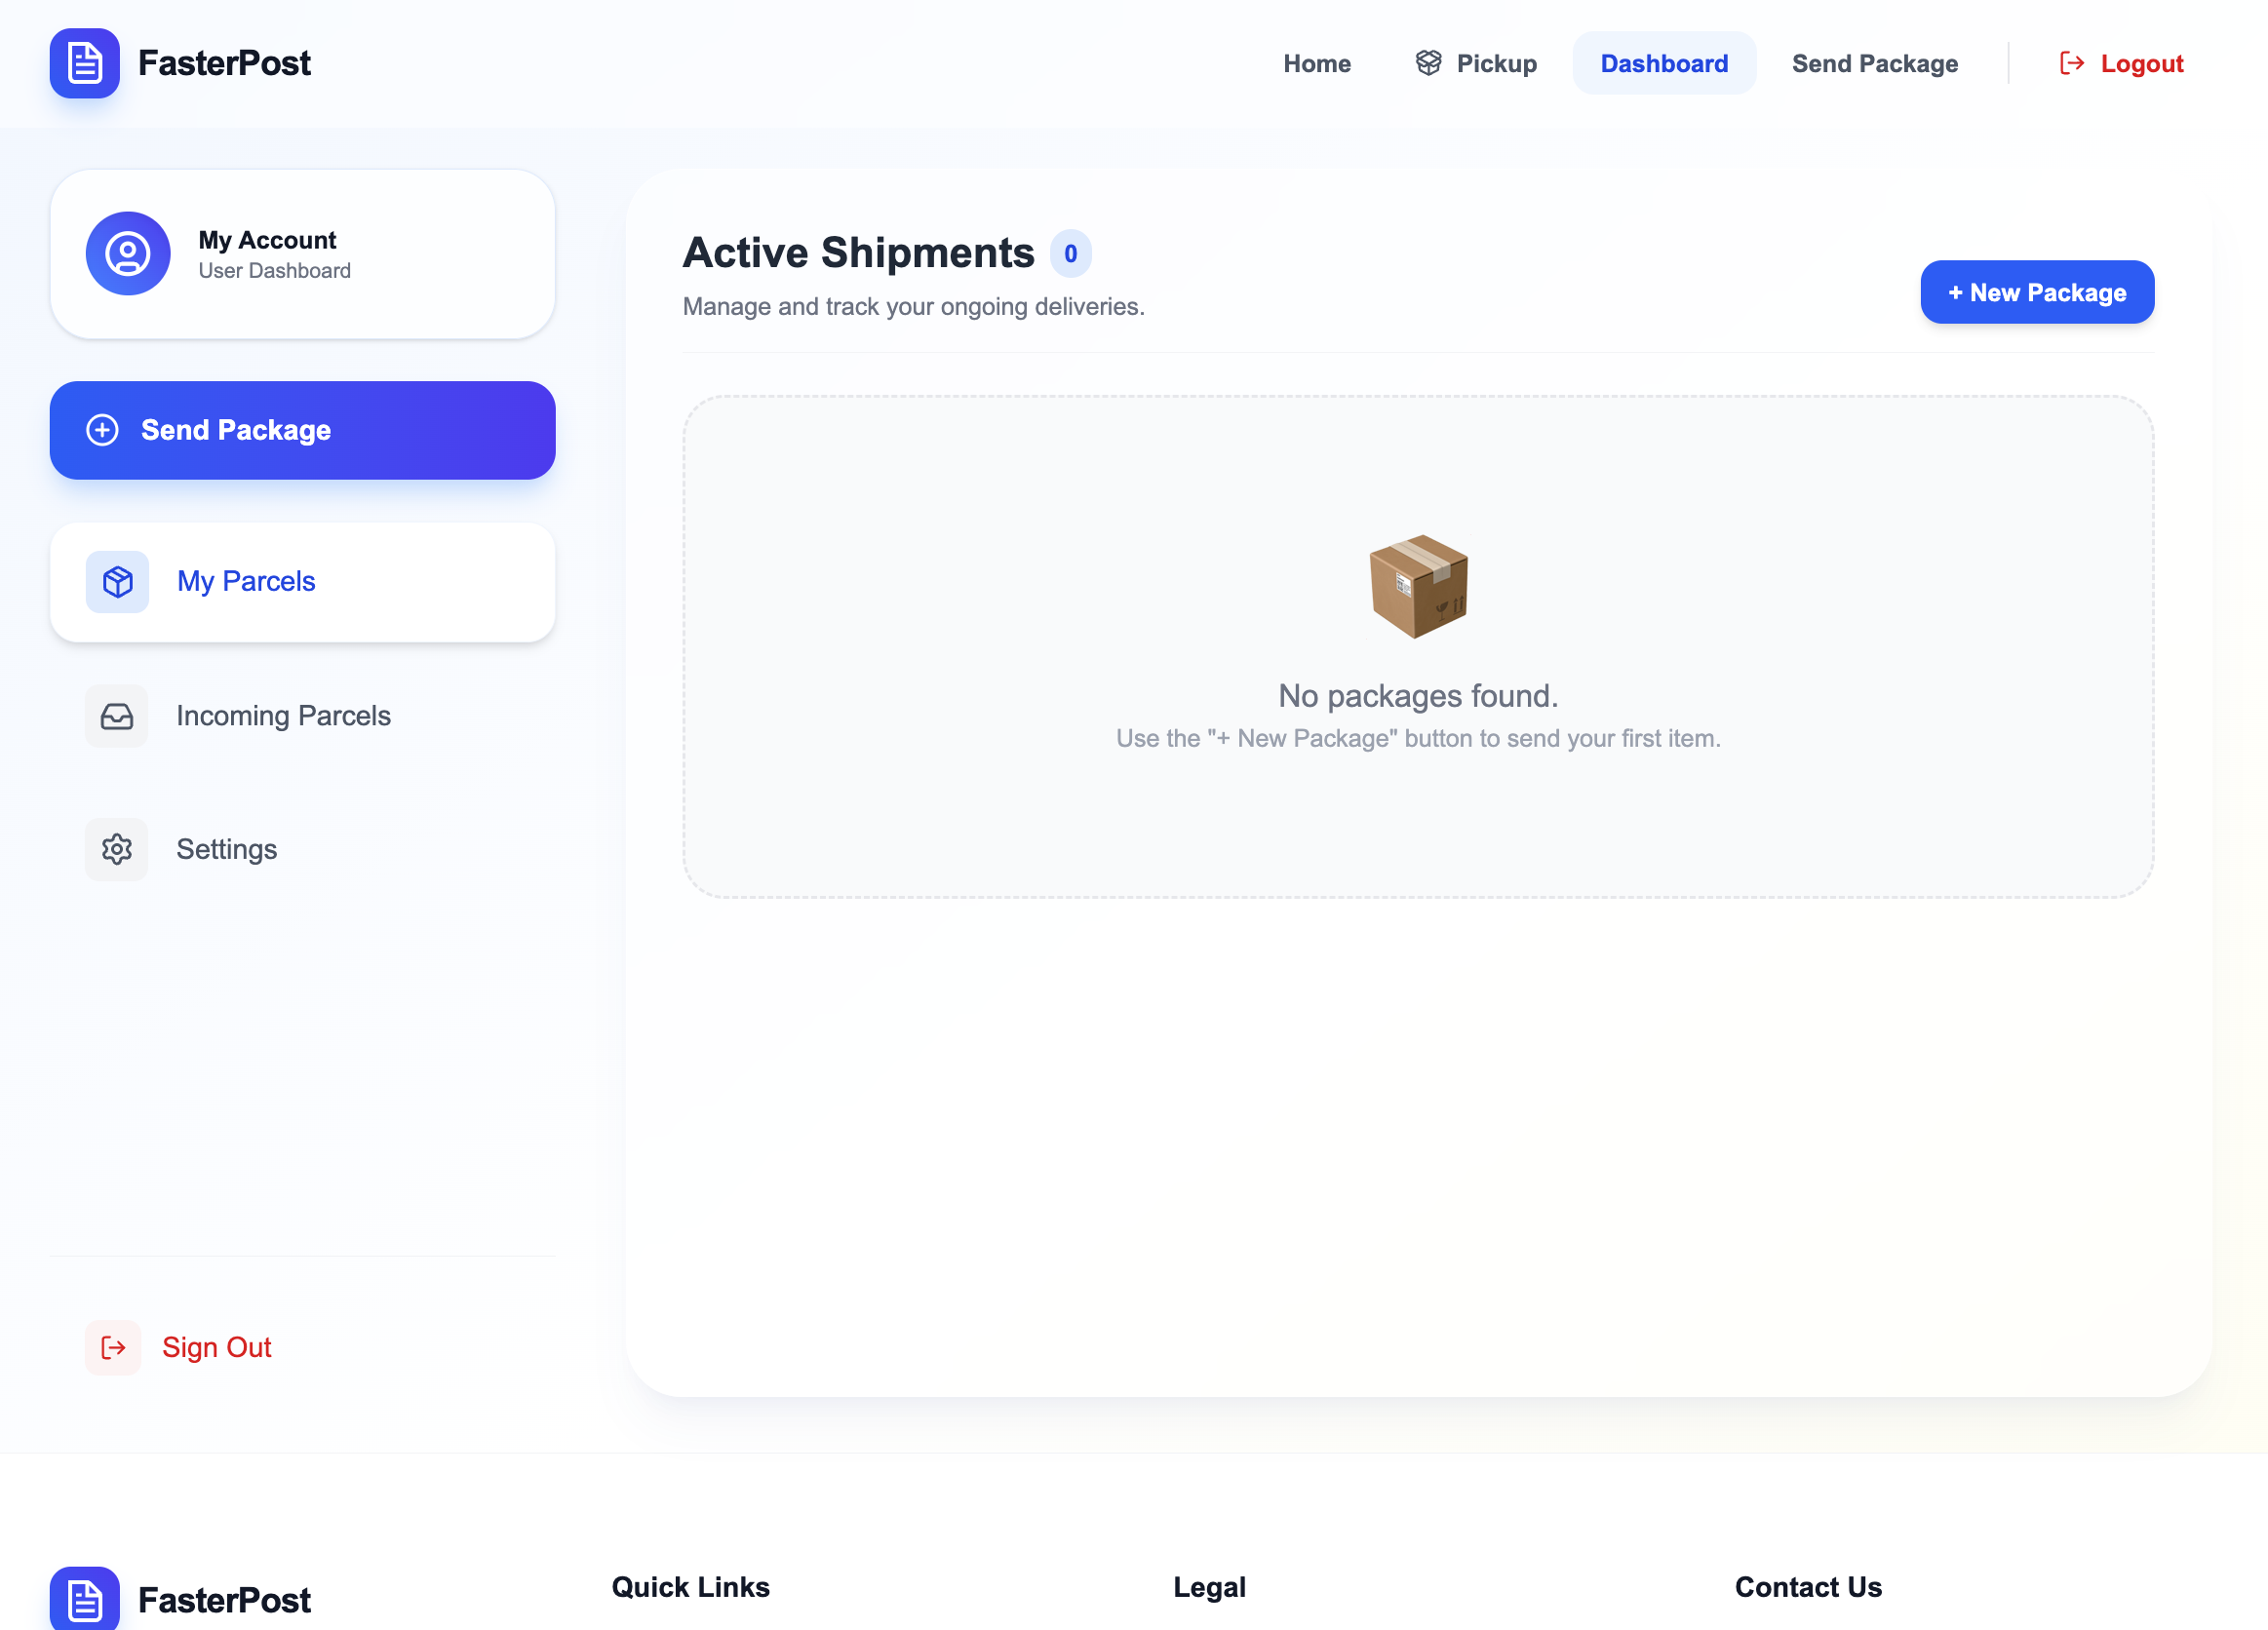
\includegraphics[width=0.7\textwidth]{../screenshots/7_user_dashboard.png}
    \caption{Dashboard użytkownika z wykorzystaniem hierarchii wizualnej.}
\end{figure}

\begin{figure}[H]
    \centering
    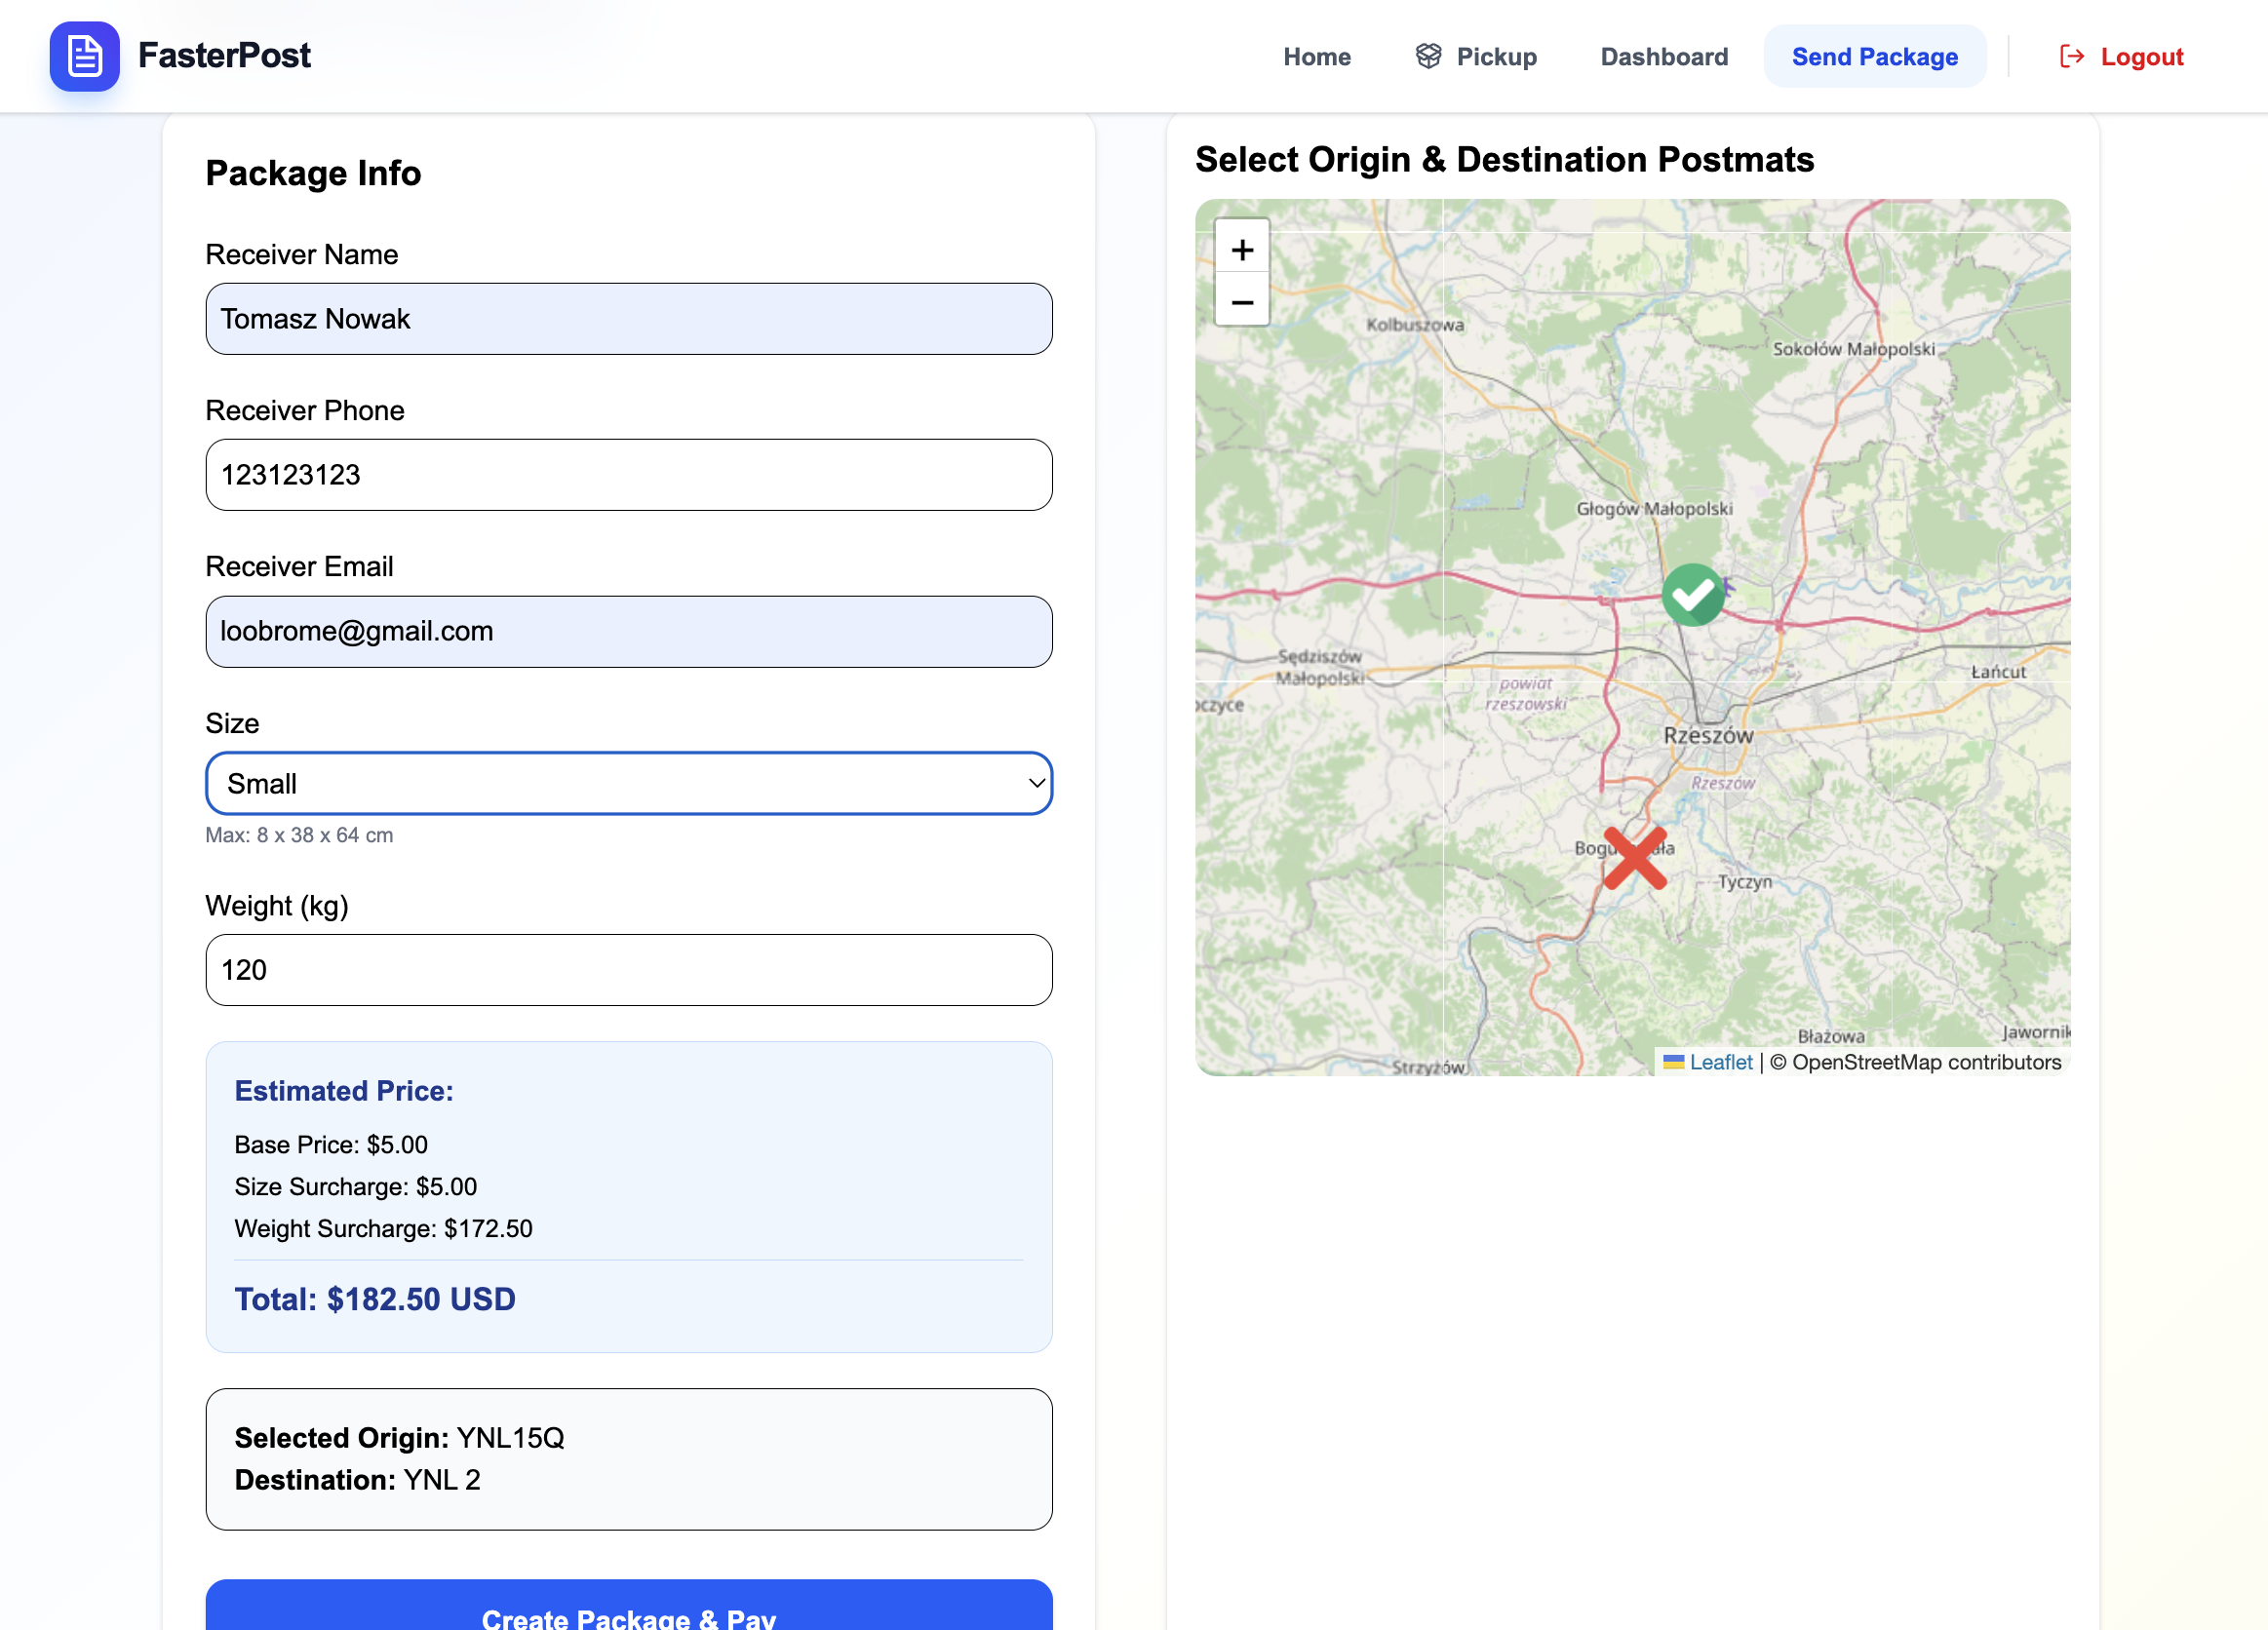
\includegraphics[width=0.45\textwidth]{../screenshots/8_normal_user_sending_package.png}
    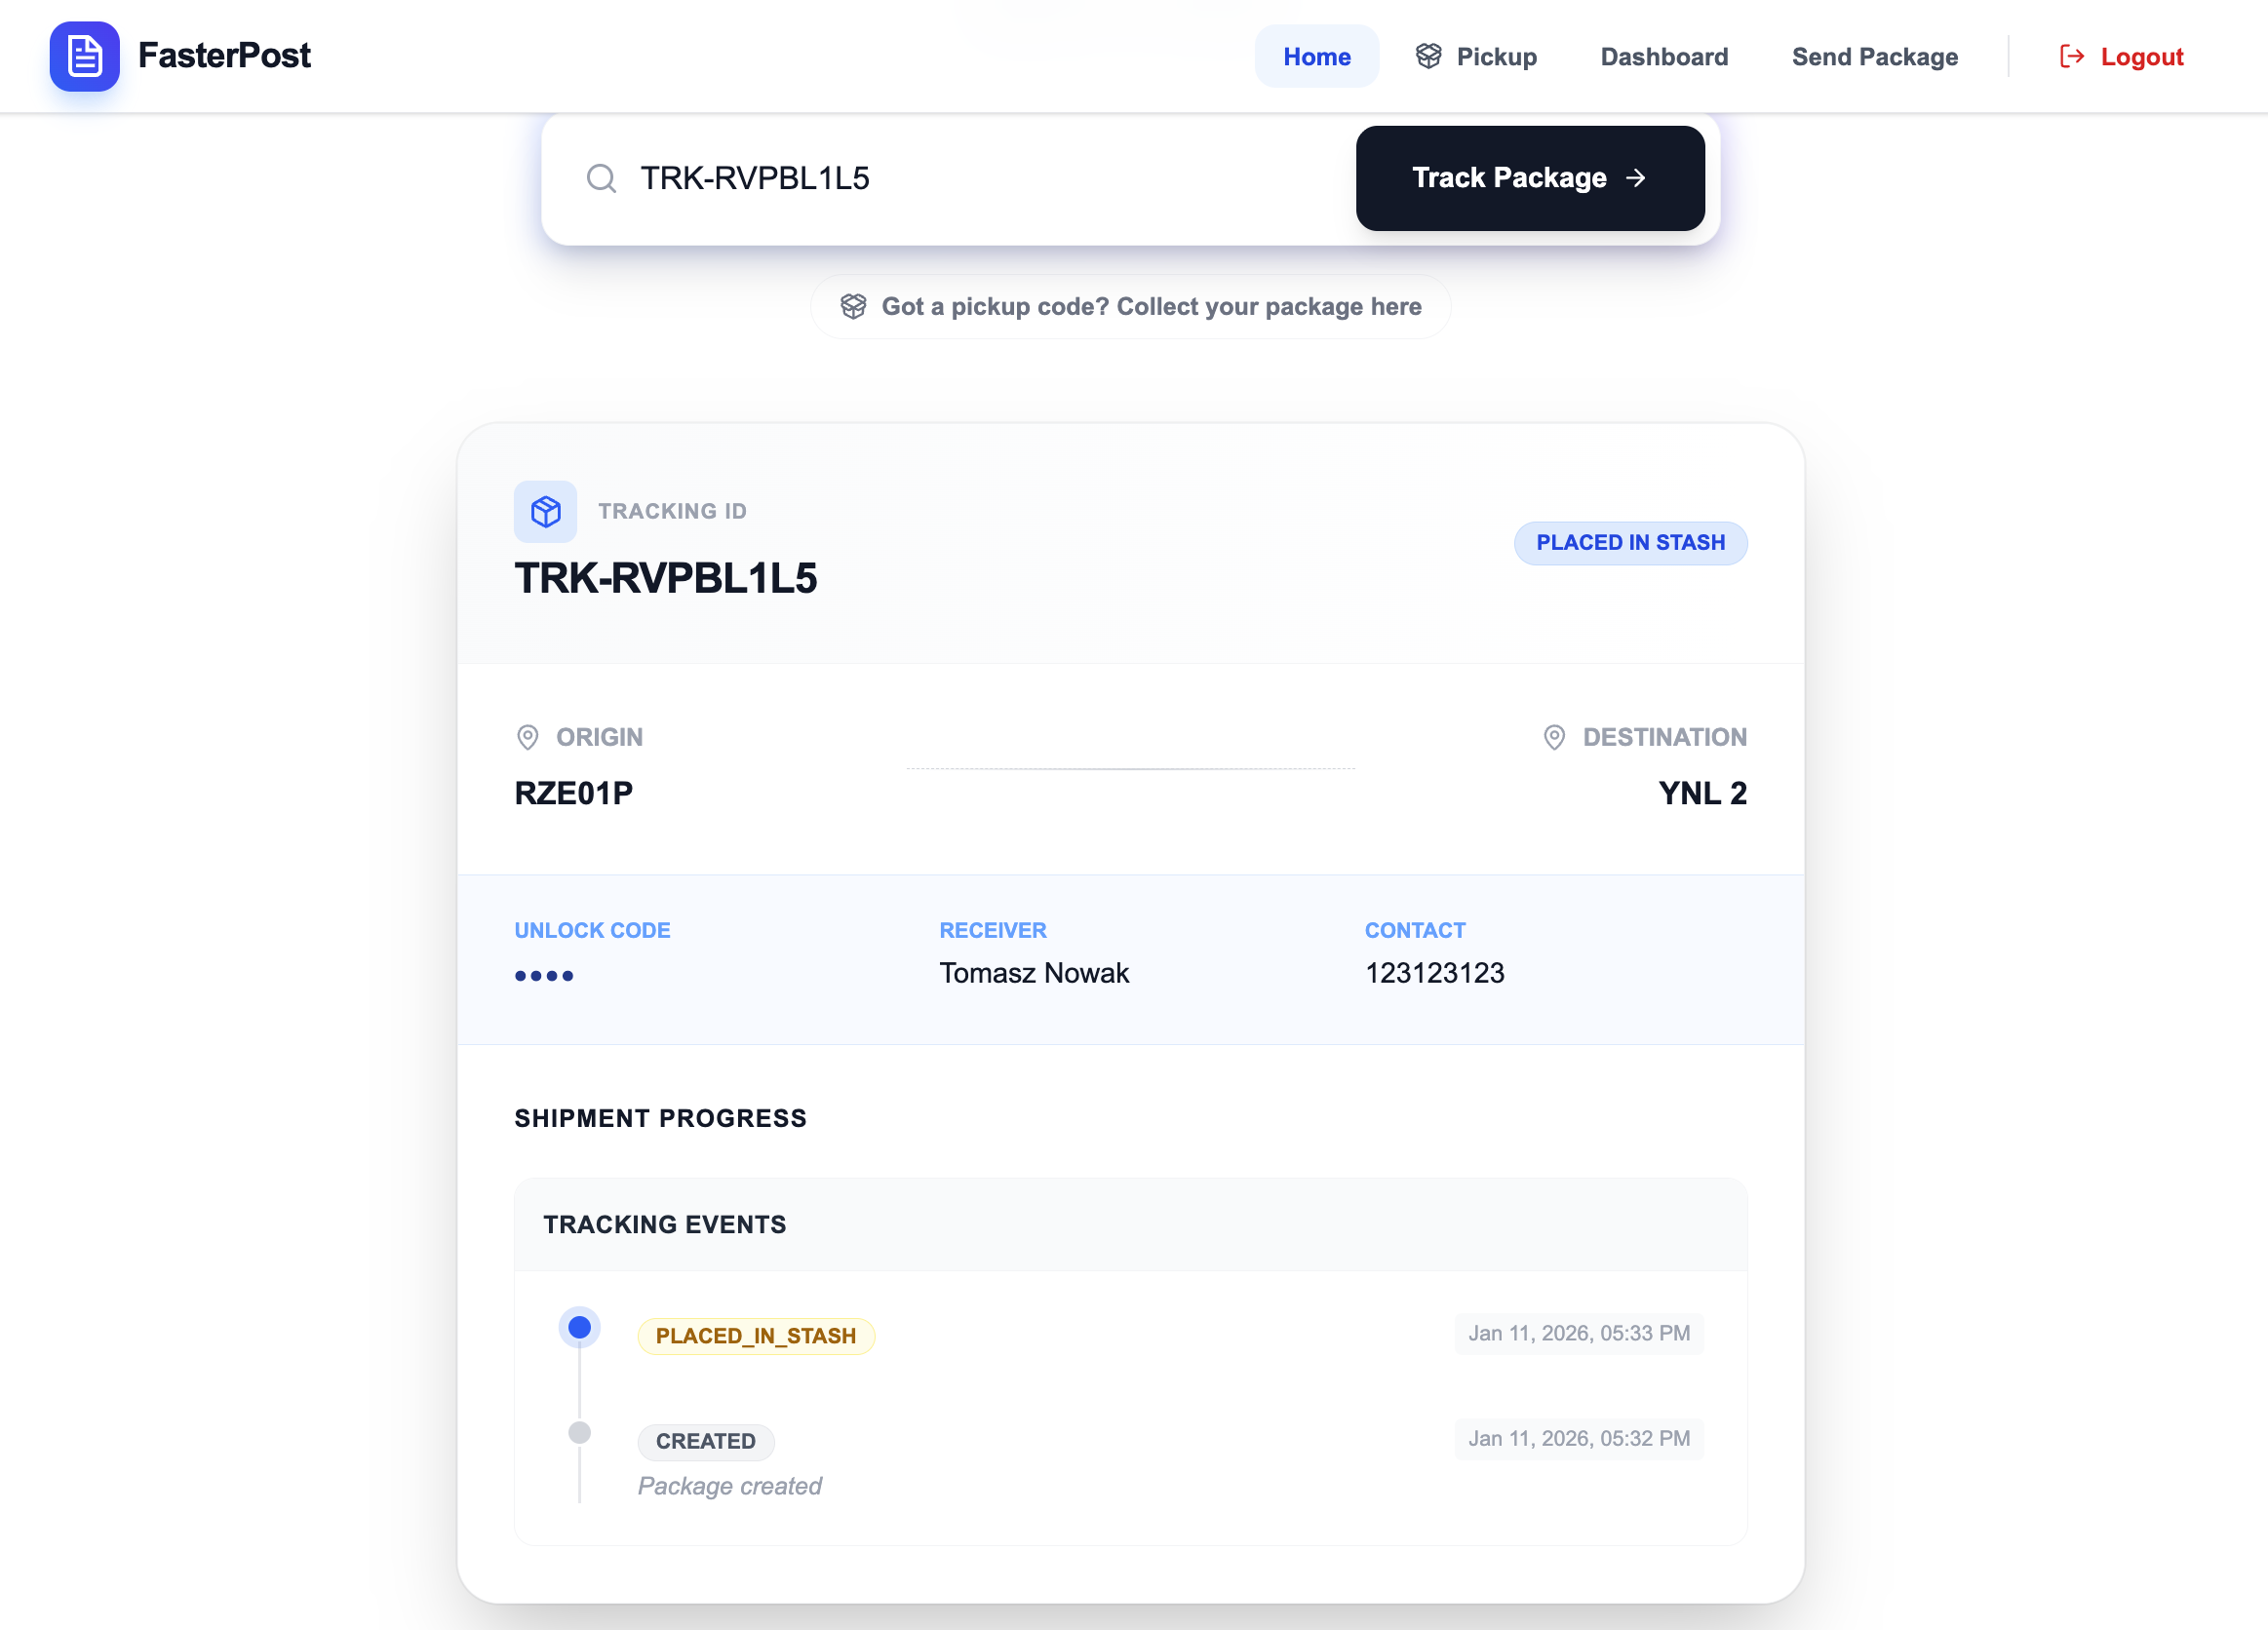
\includegraphics[width=0.45\textwidth]{../screenshots/9_tracking_package.png}
    \caption{Proces nadawania przesyłki oraz widok śledzenia z wskaźnikiem postępu.}
\end{figure}

\begin{figure}[H]
    \centering
    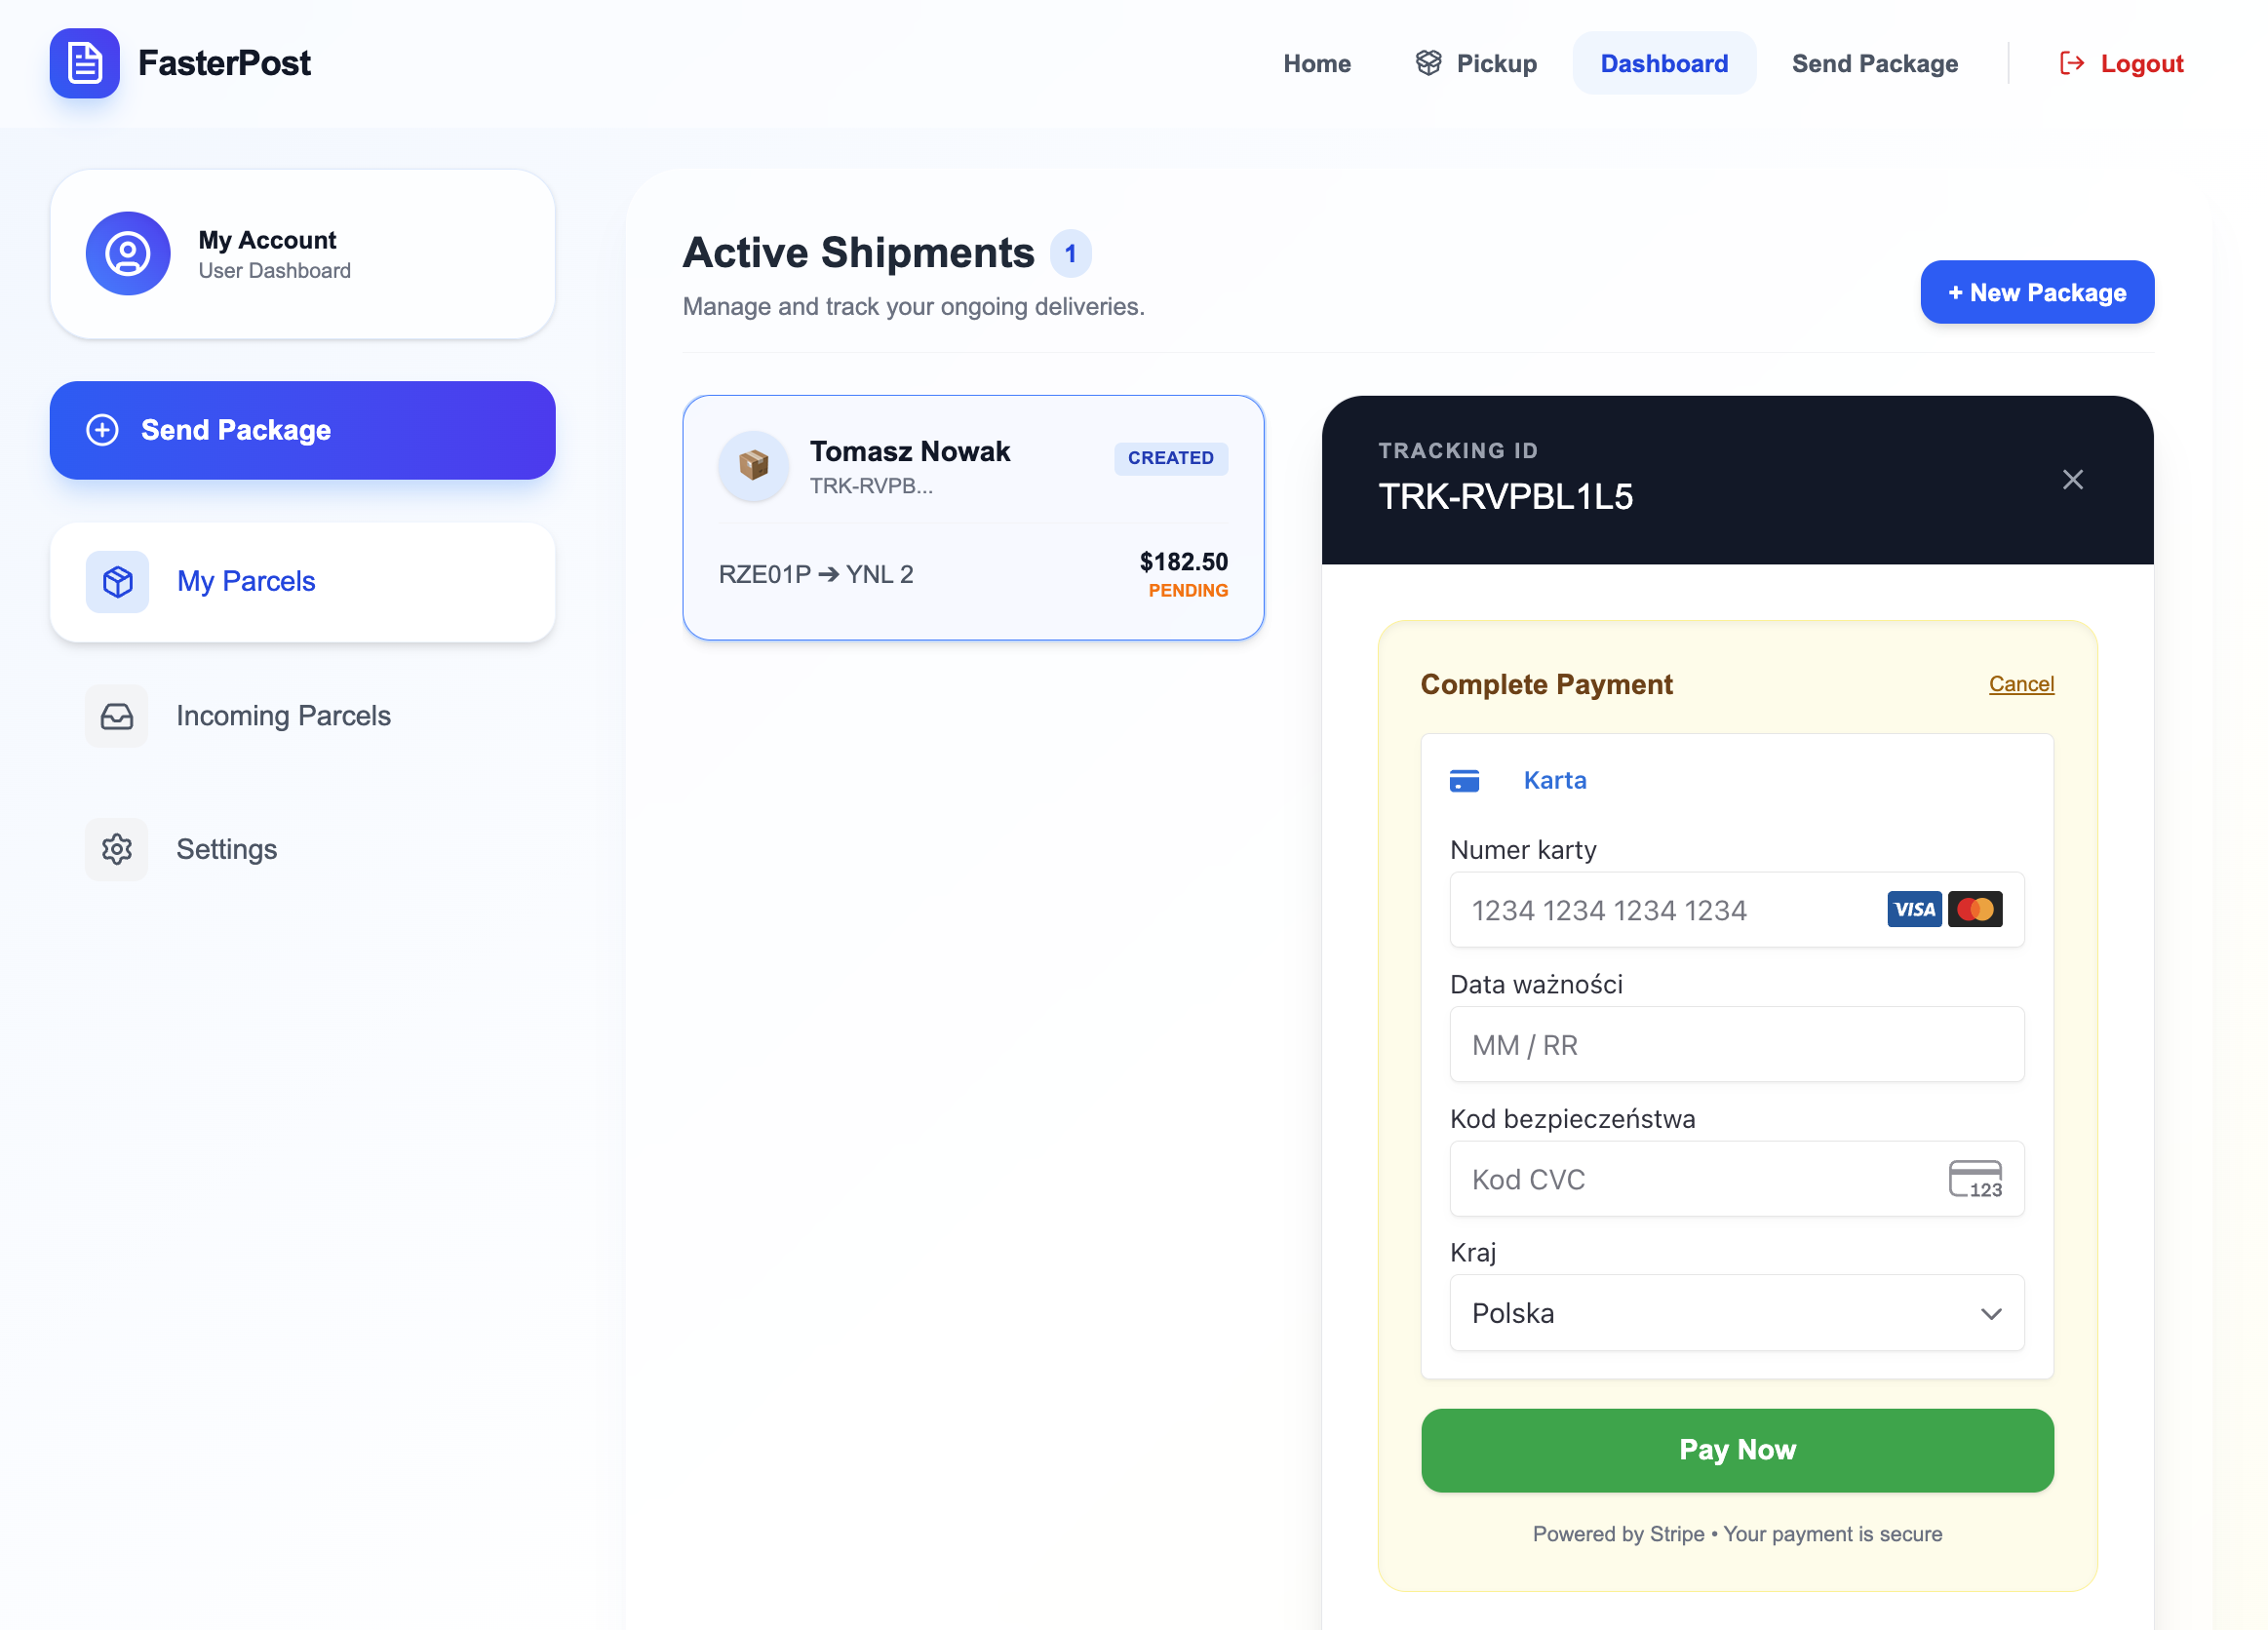
\includegraphics[width=0.45\textwidth]{../screenshots/8_normal_user_payment.png}
    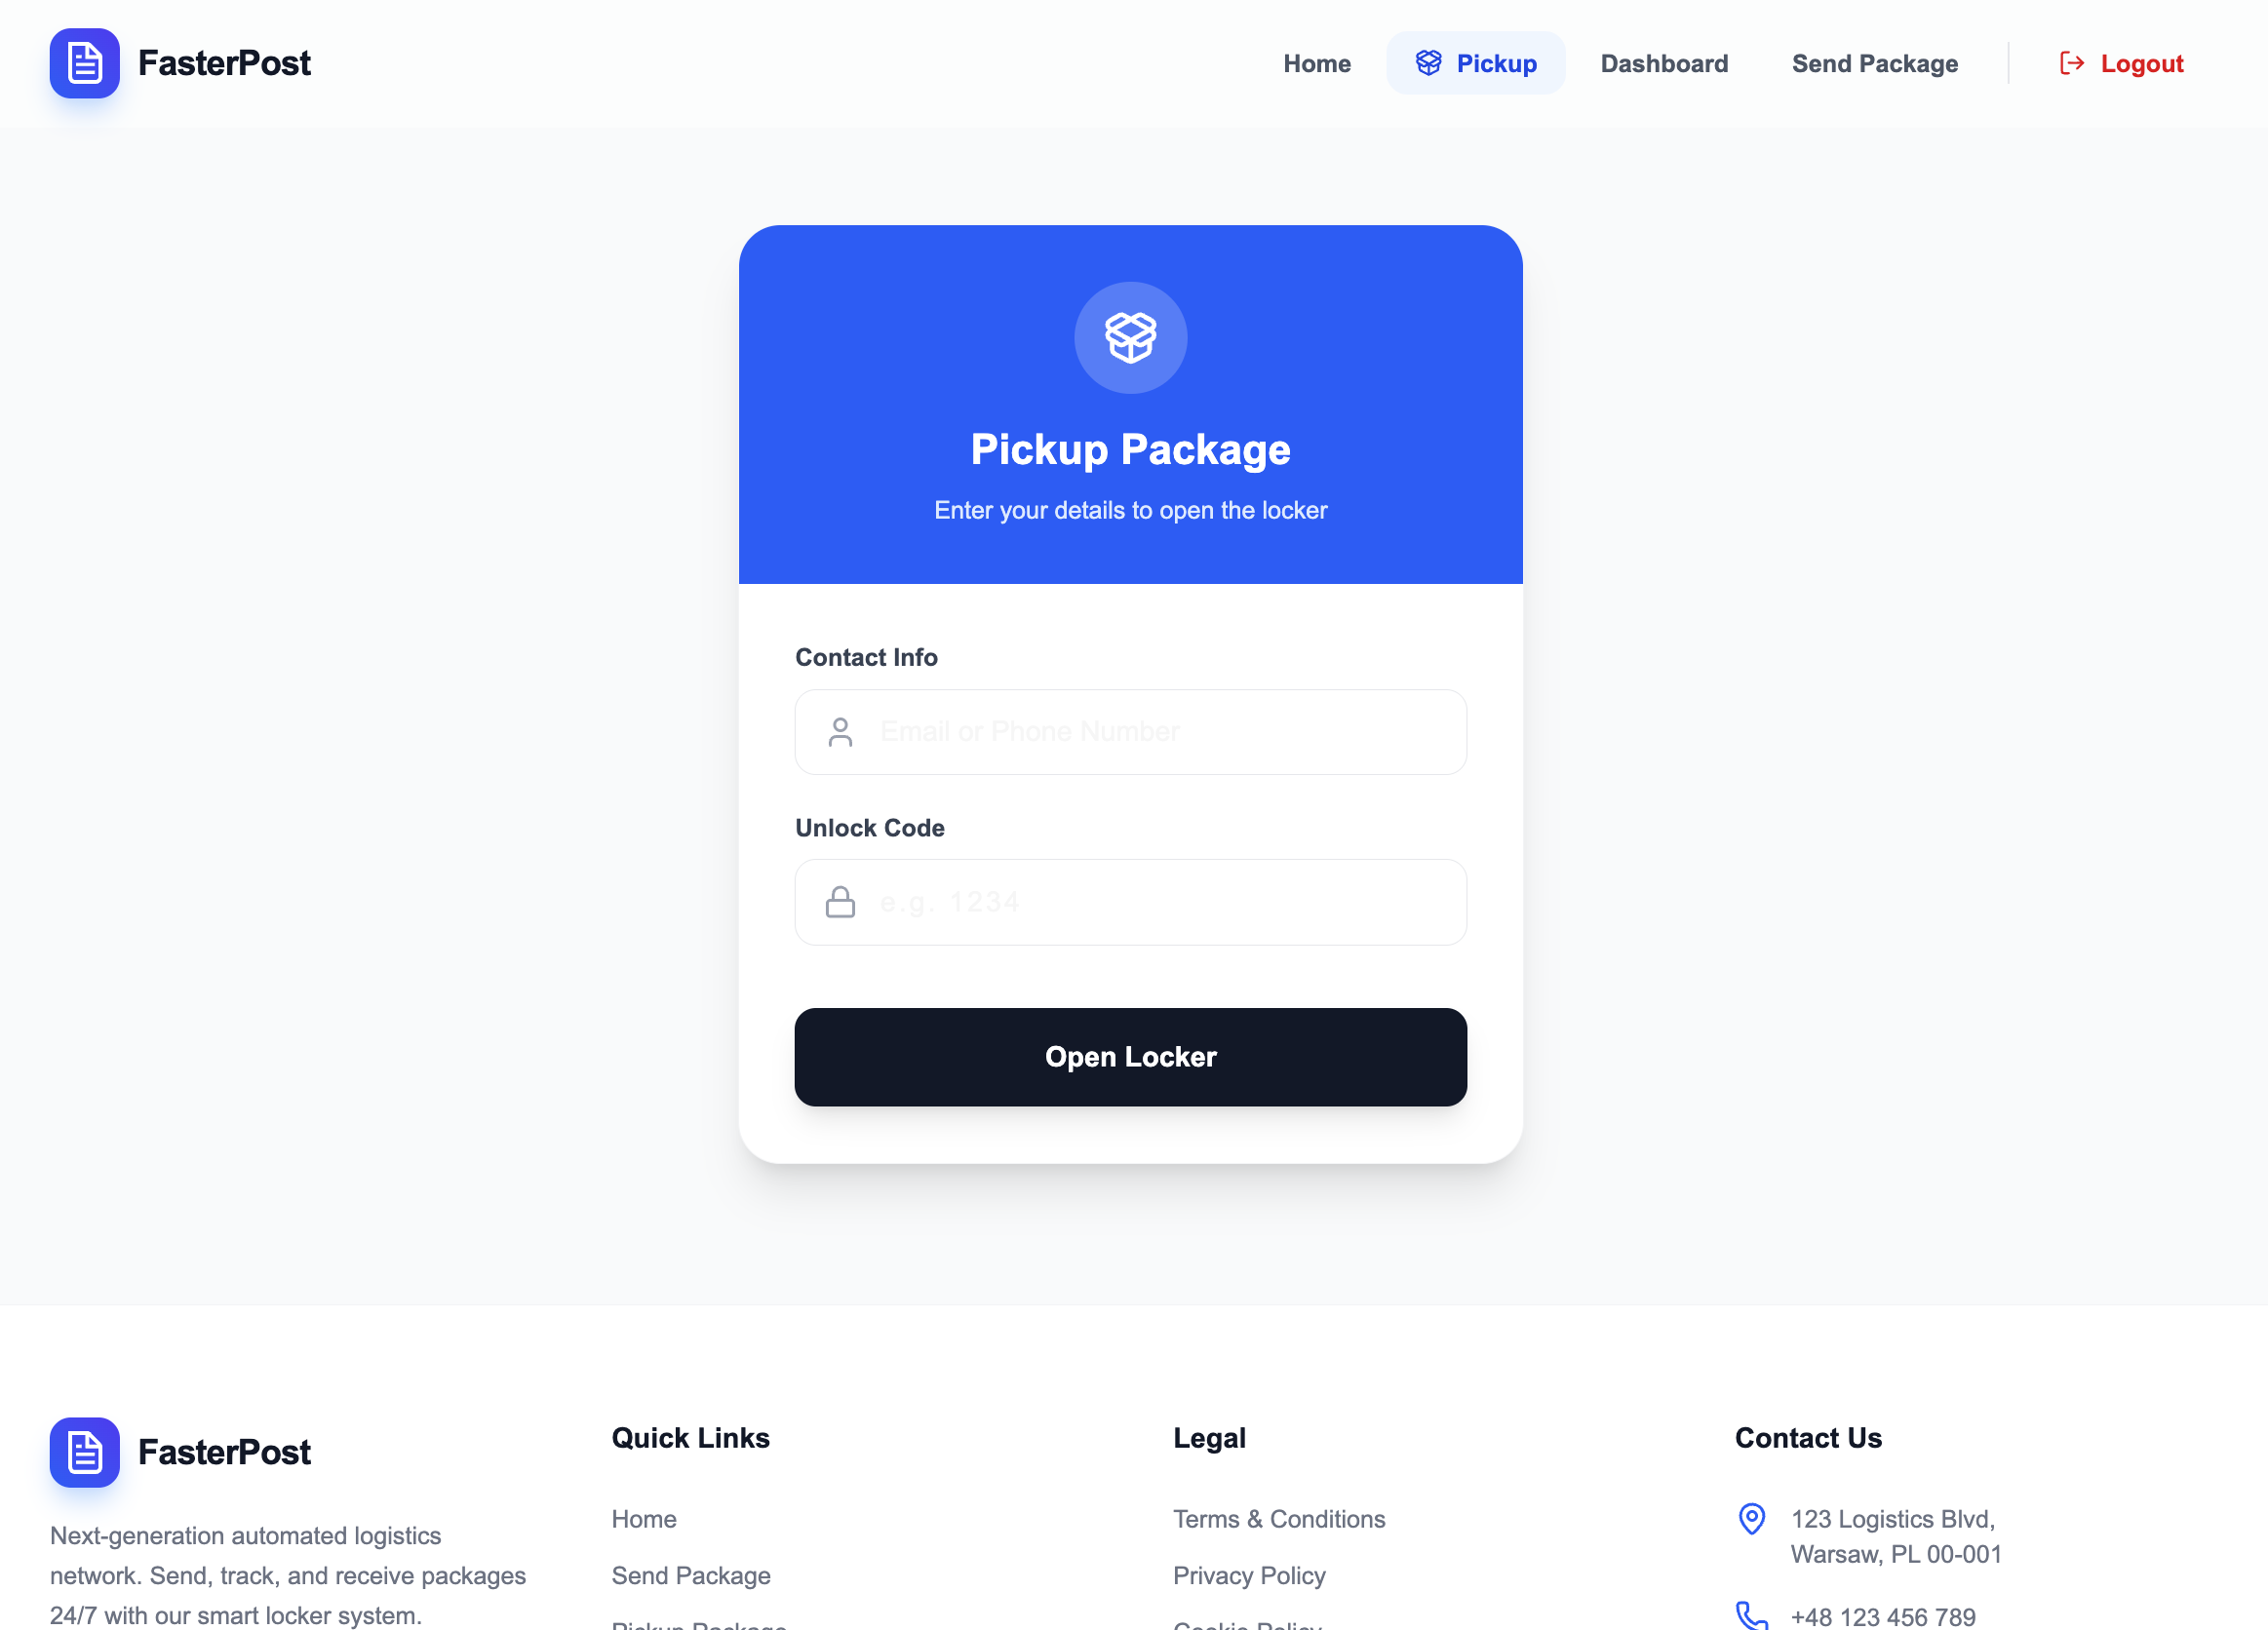
\includegraphics[width=0.45\textwidth]{../screenshots/10_pickup_package.png}
    \caption{Ekran płatności oraz interfejs odbioru paczki.}
\end{figure}

\subsection{Panel biznesowy}
Dla użytkowników biznesowych zastosowano menu boczne (Side Navigation) oraz rozbudowane moduły statystyk i masowej obsługi zamówień.

\begin{figure}[H]
    \centering
    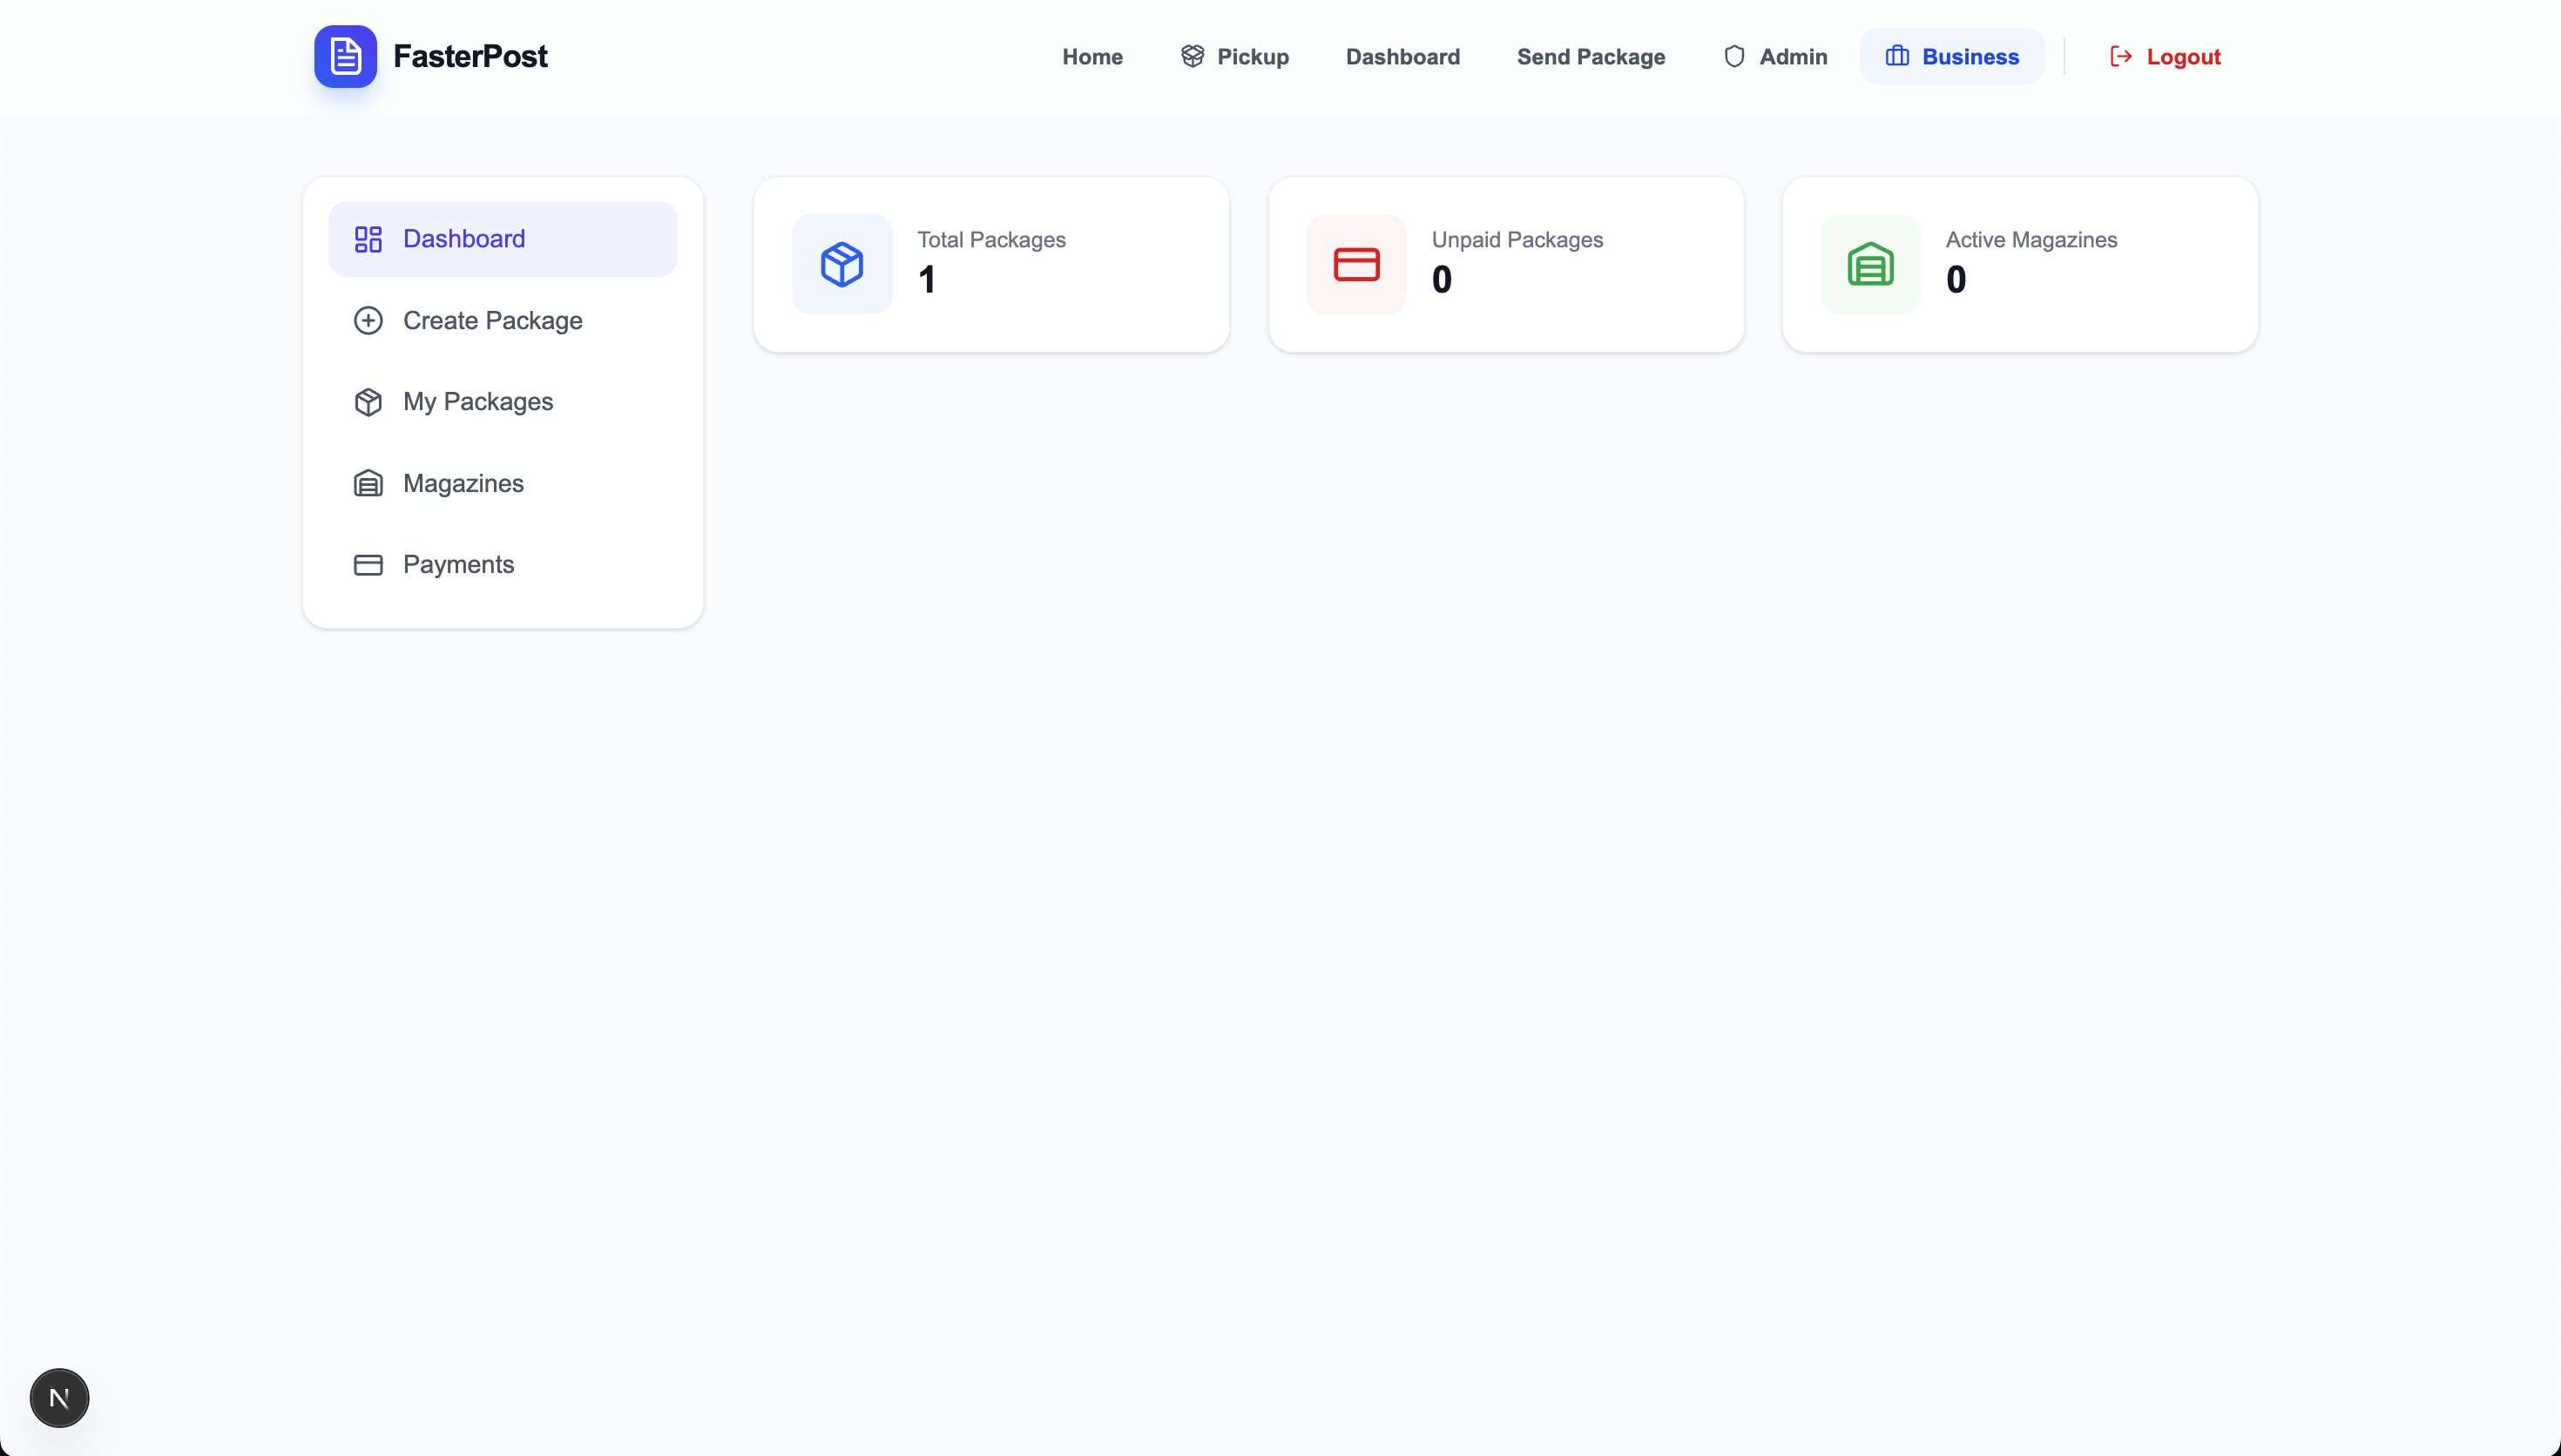
\includegraphics[width=0.7\textwidth]{../screenshots/6_business_dashboard.png}
    \caption{Panel biznesowy z menu bocznym i statystykami.}
\end{figure}

\begin{figure}[H]
    \centering
    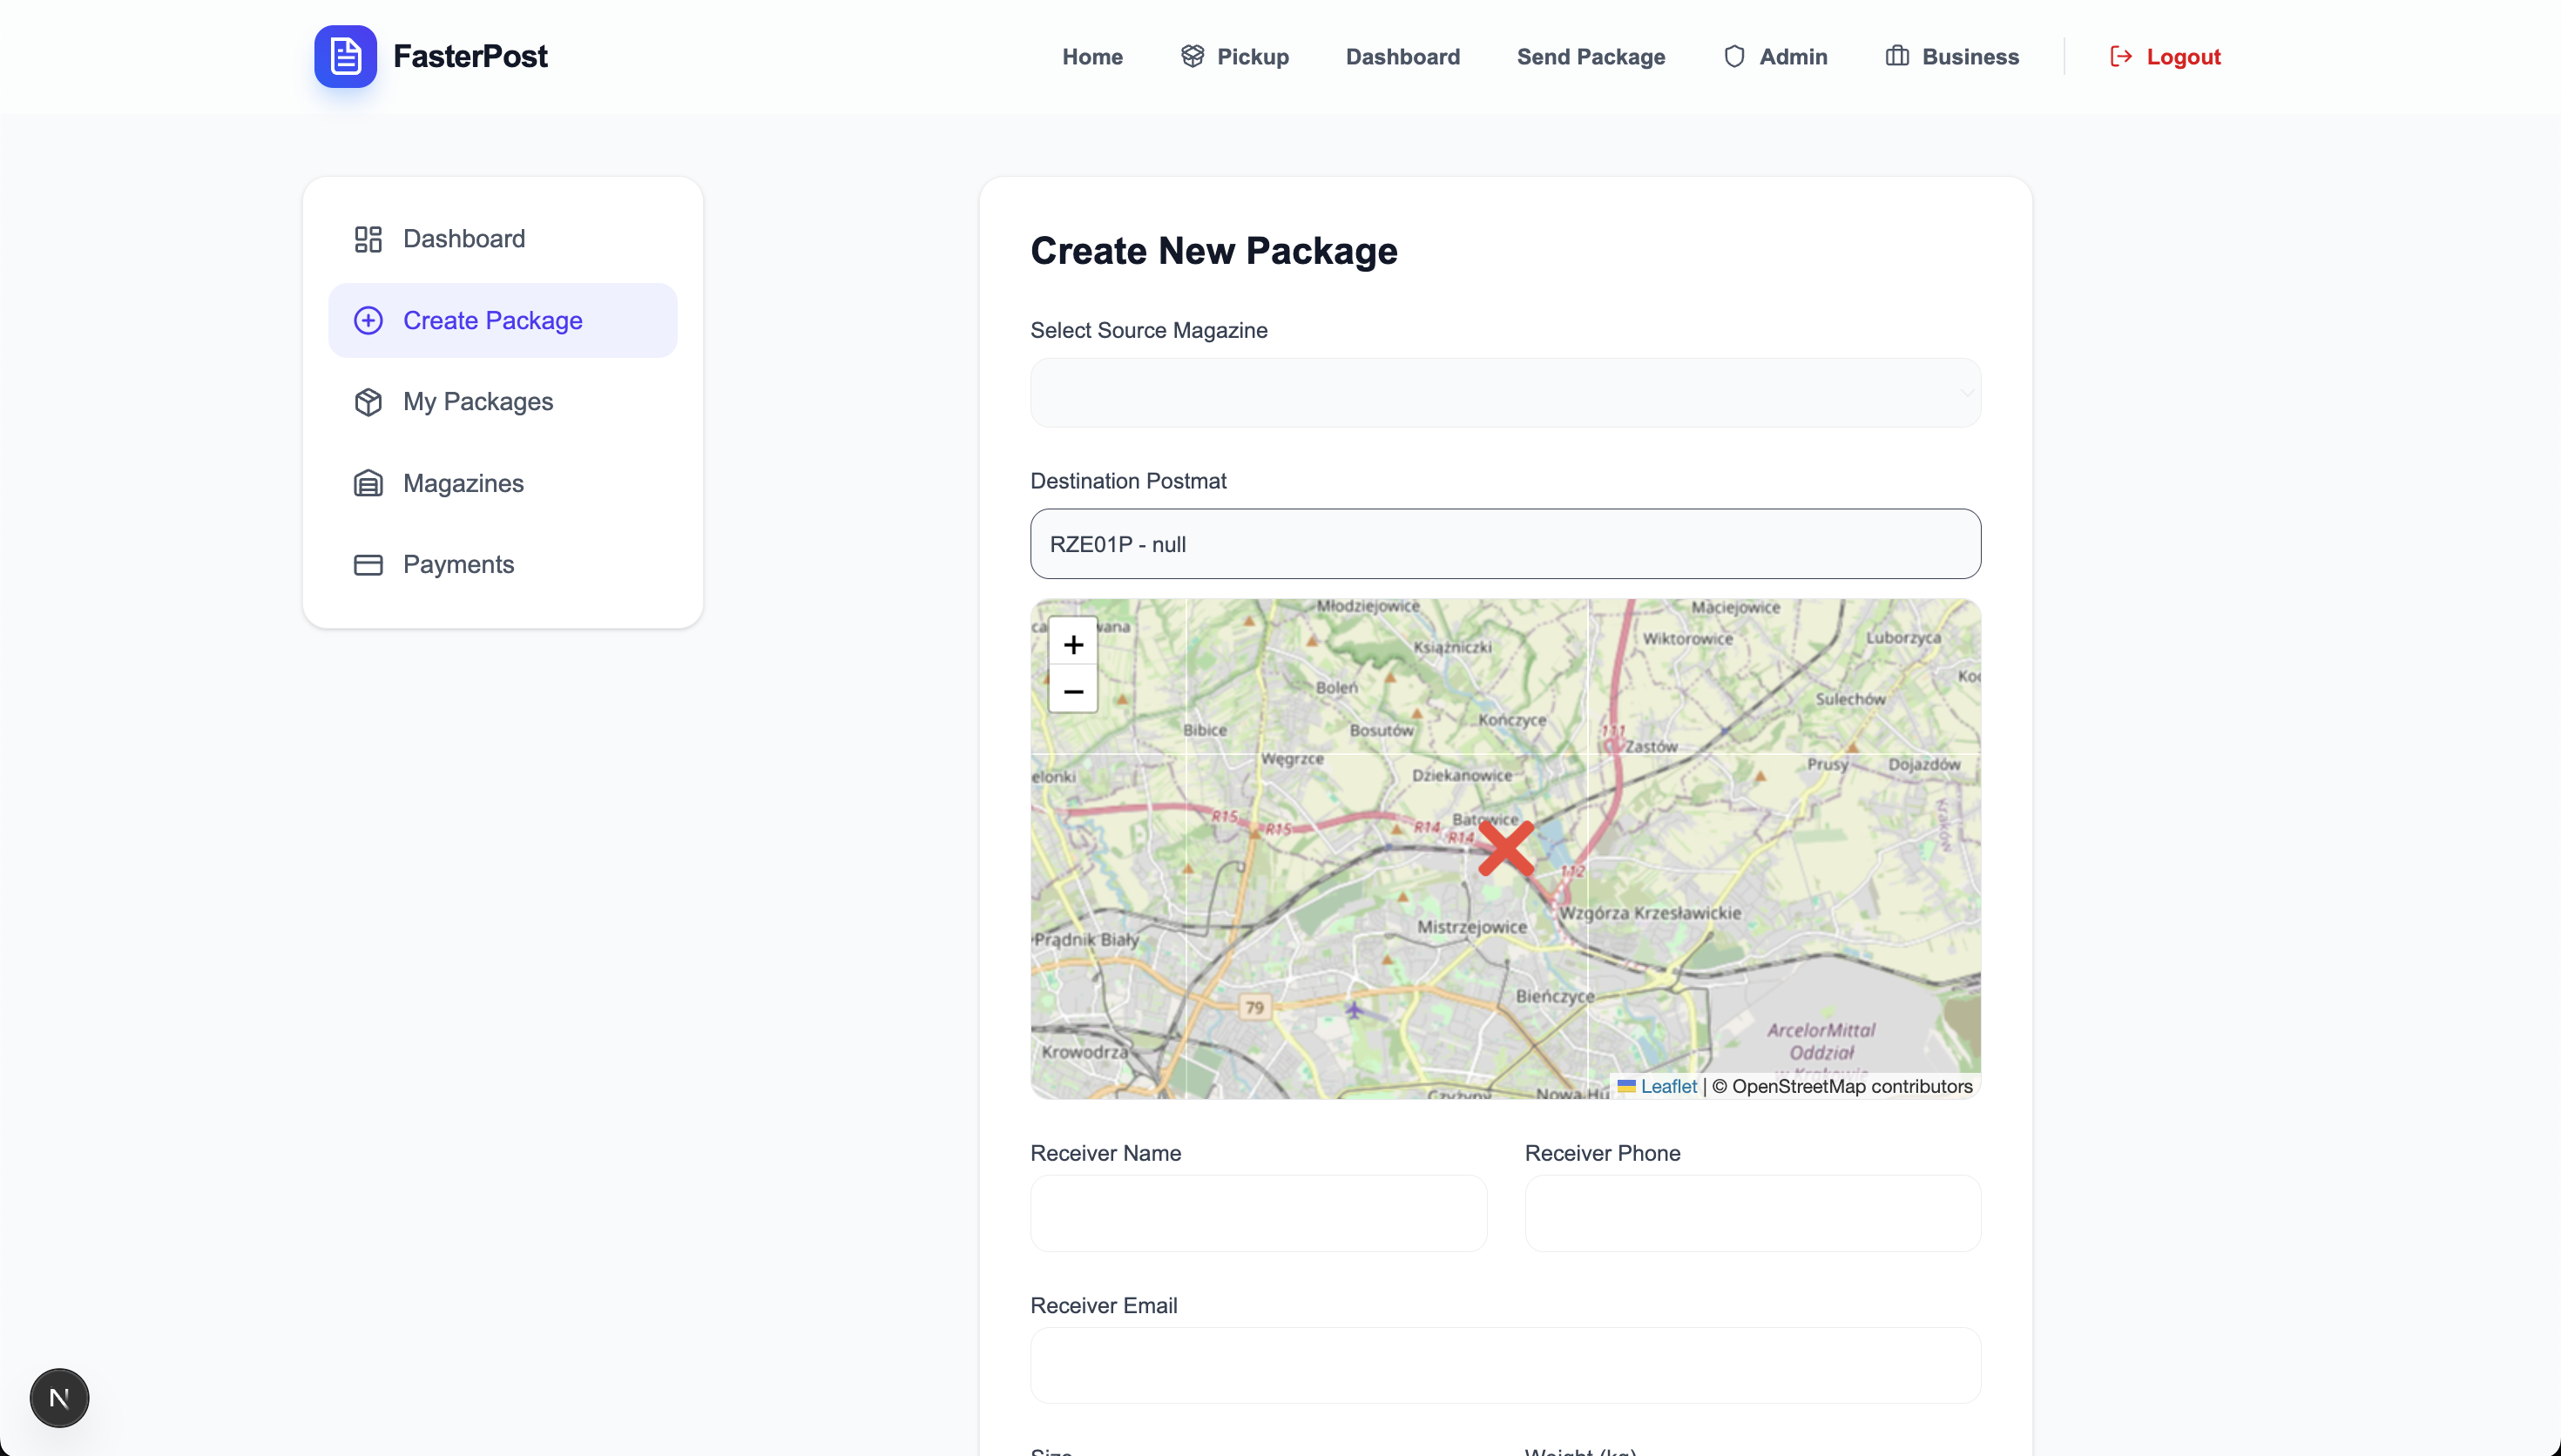
\includegraphics[width=0.7\textwidth]{../screenshots/6_business_sending_packages.png}
    \caption{Formularz masowego nadawania przesyłek dla sektora B2B.}
\end{figure}

\section{Zarządzanie systemem i logistyka}
Panele administracyjne oraz logistyczne skupiają się na wydajnym zarządzaniu infrastrukturą i przepływem towarów przy użyciu tabel, list oraz map.

\begin{figure}[H]
    \centering
    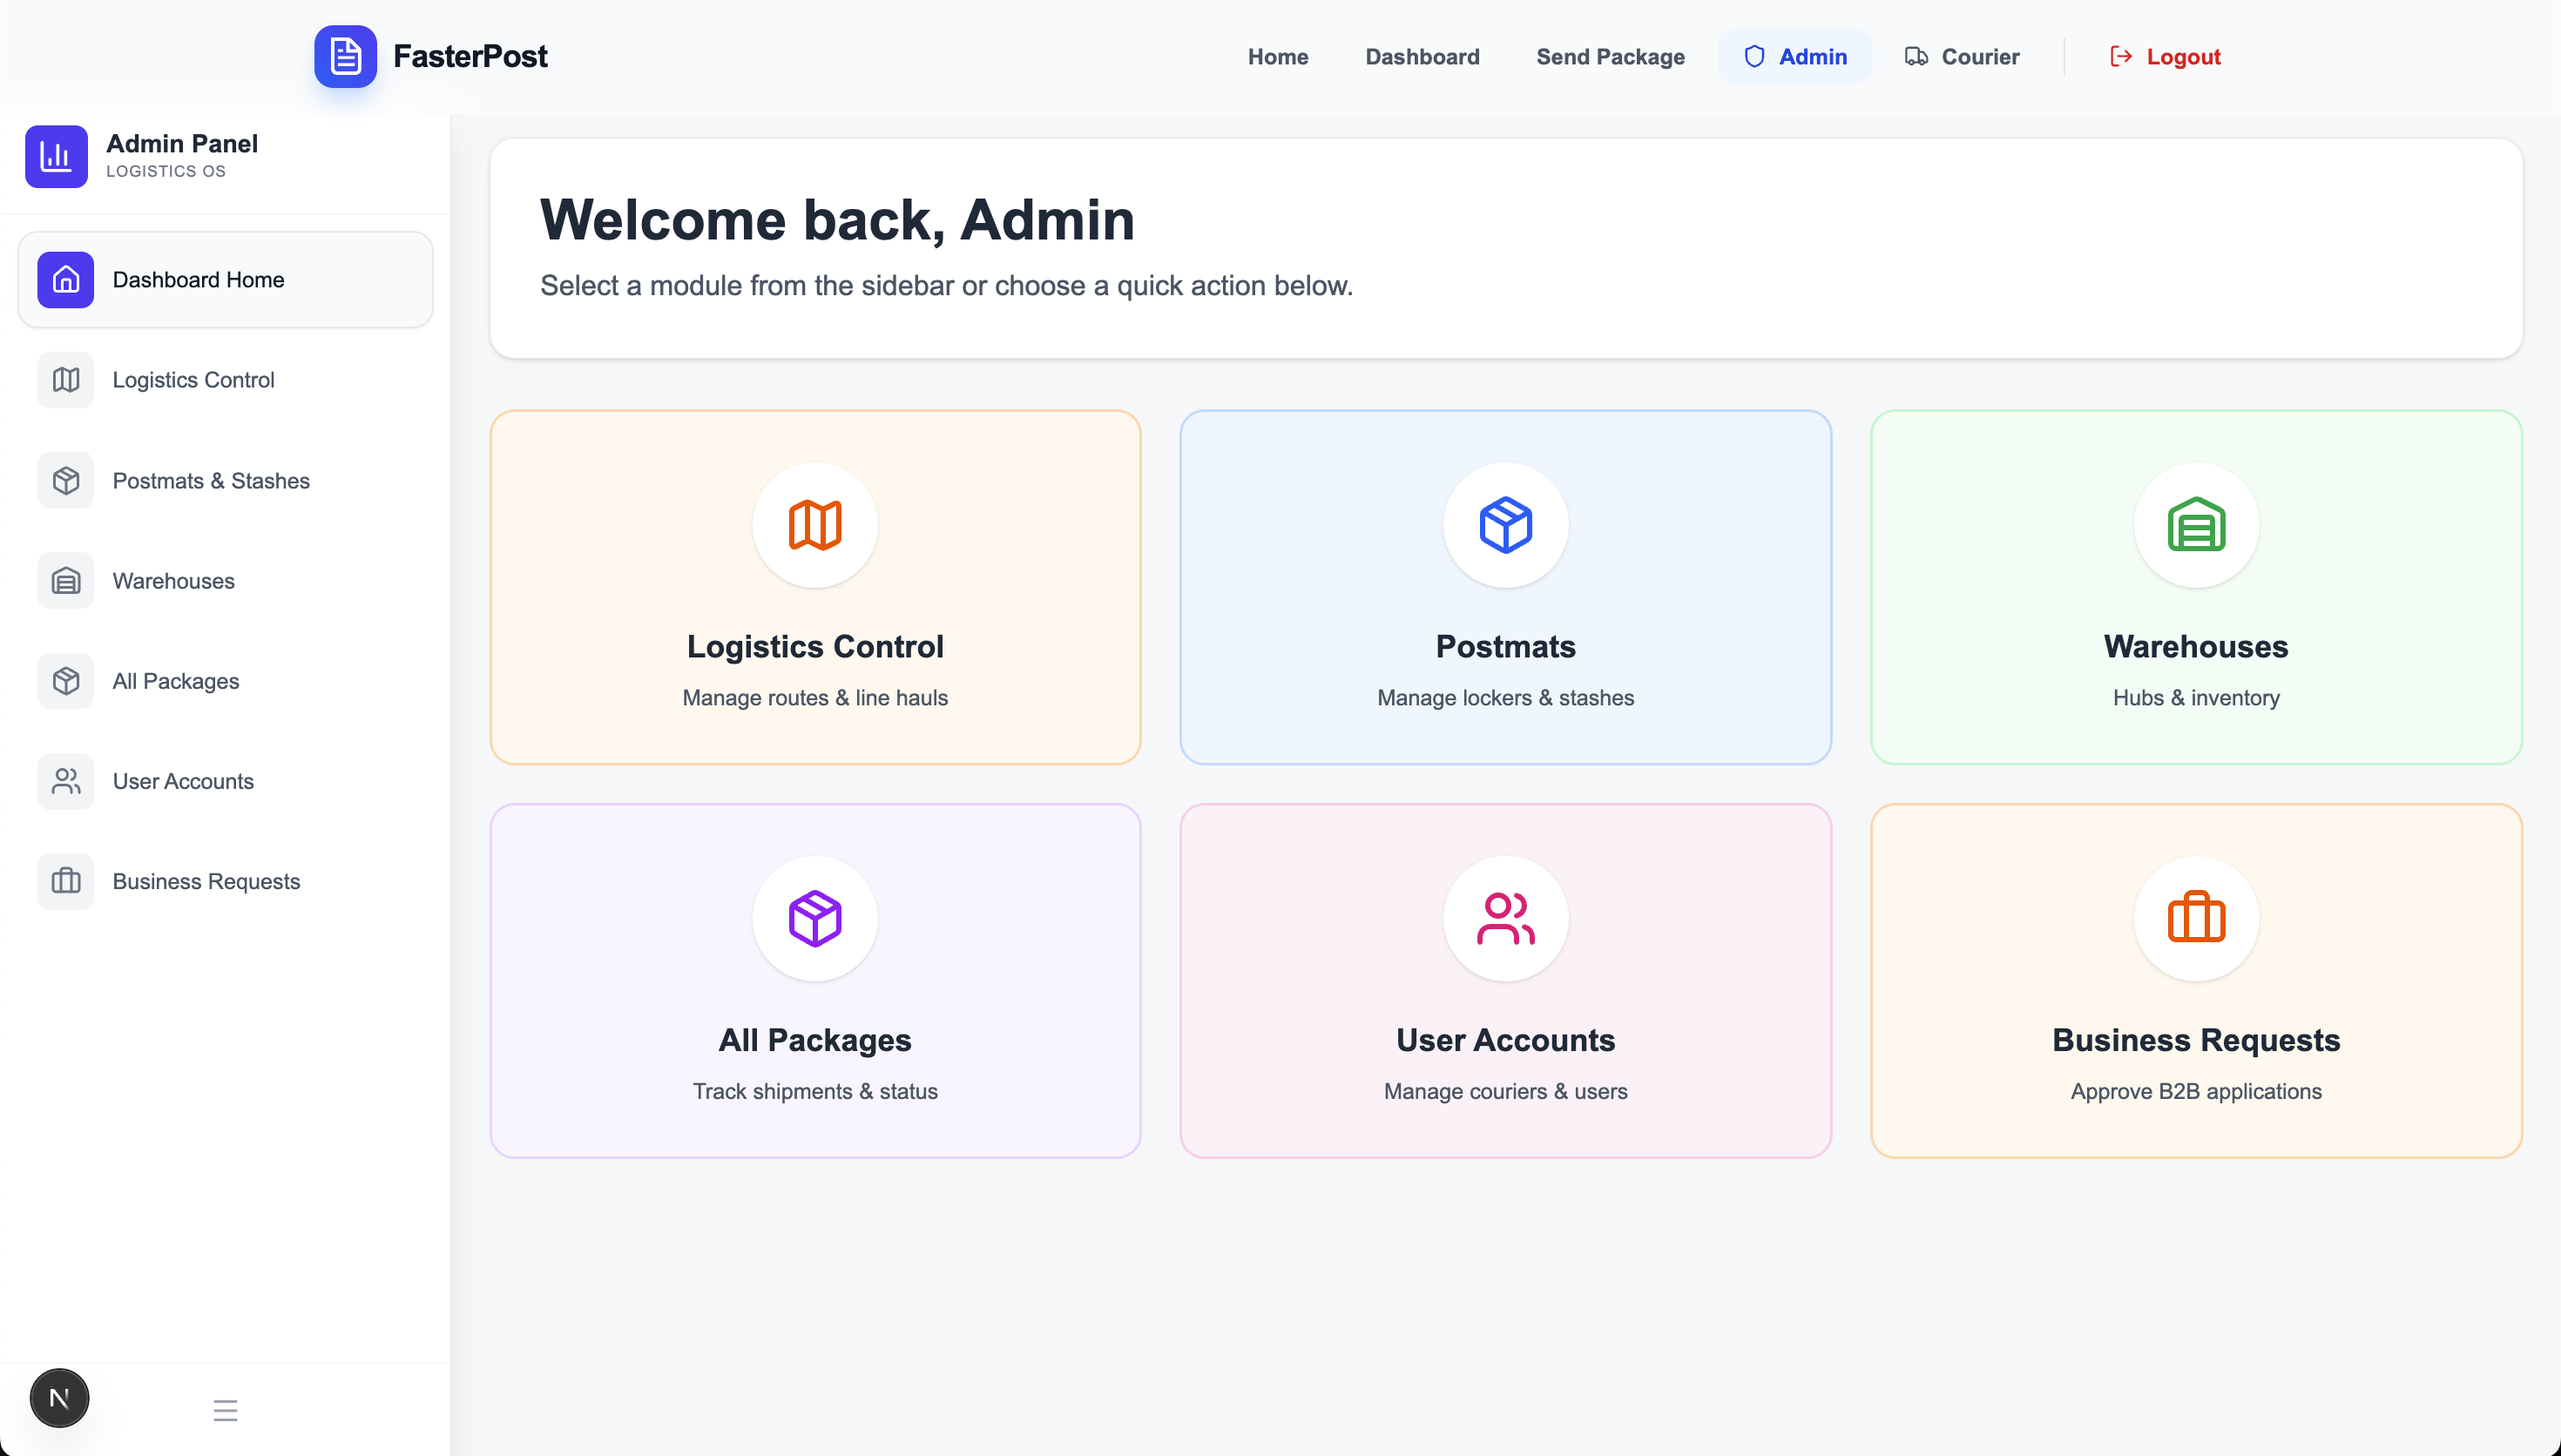
\includegraphics[width=0.7\textwidth]{../screenshots/11_admin_dashboard.png}
    \caption{Główny pulpit administratora systemu.}
\end{figure}

\begin{figure}[H]
    \centering
    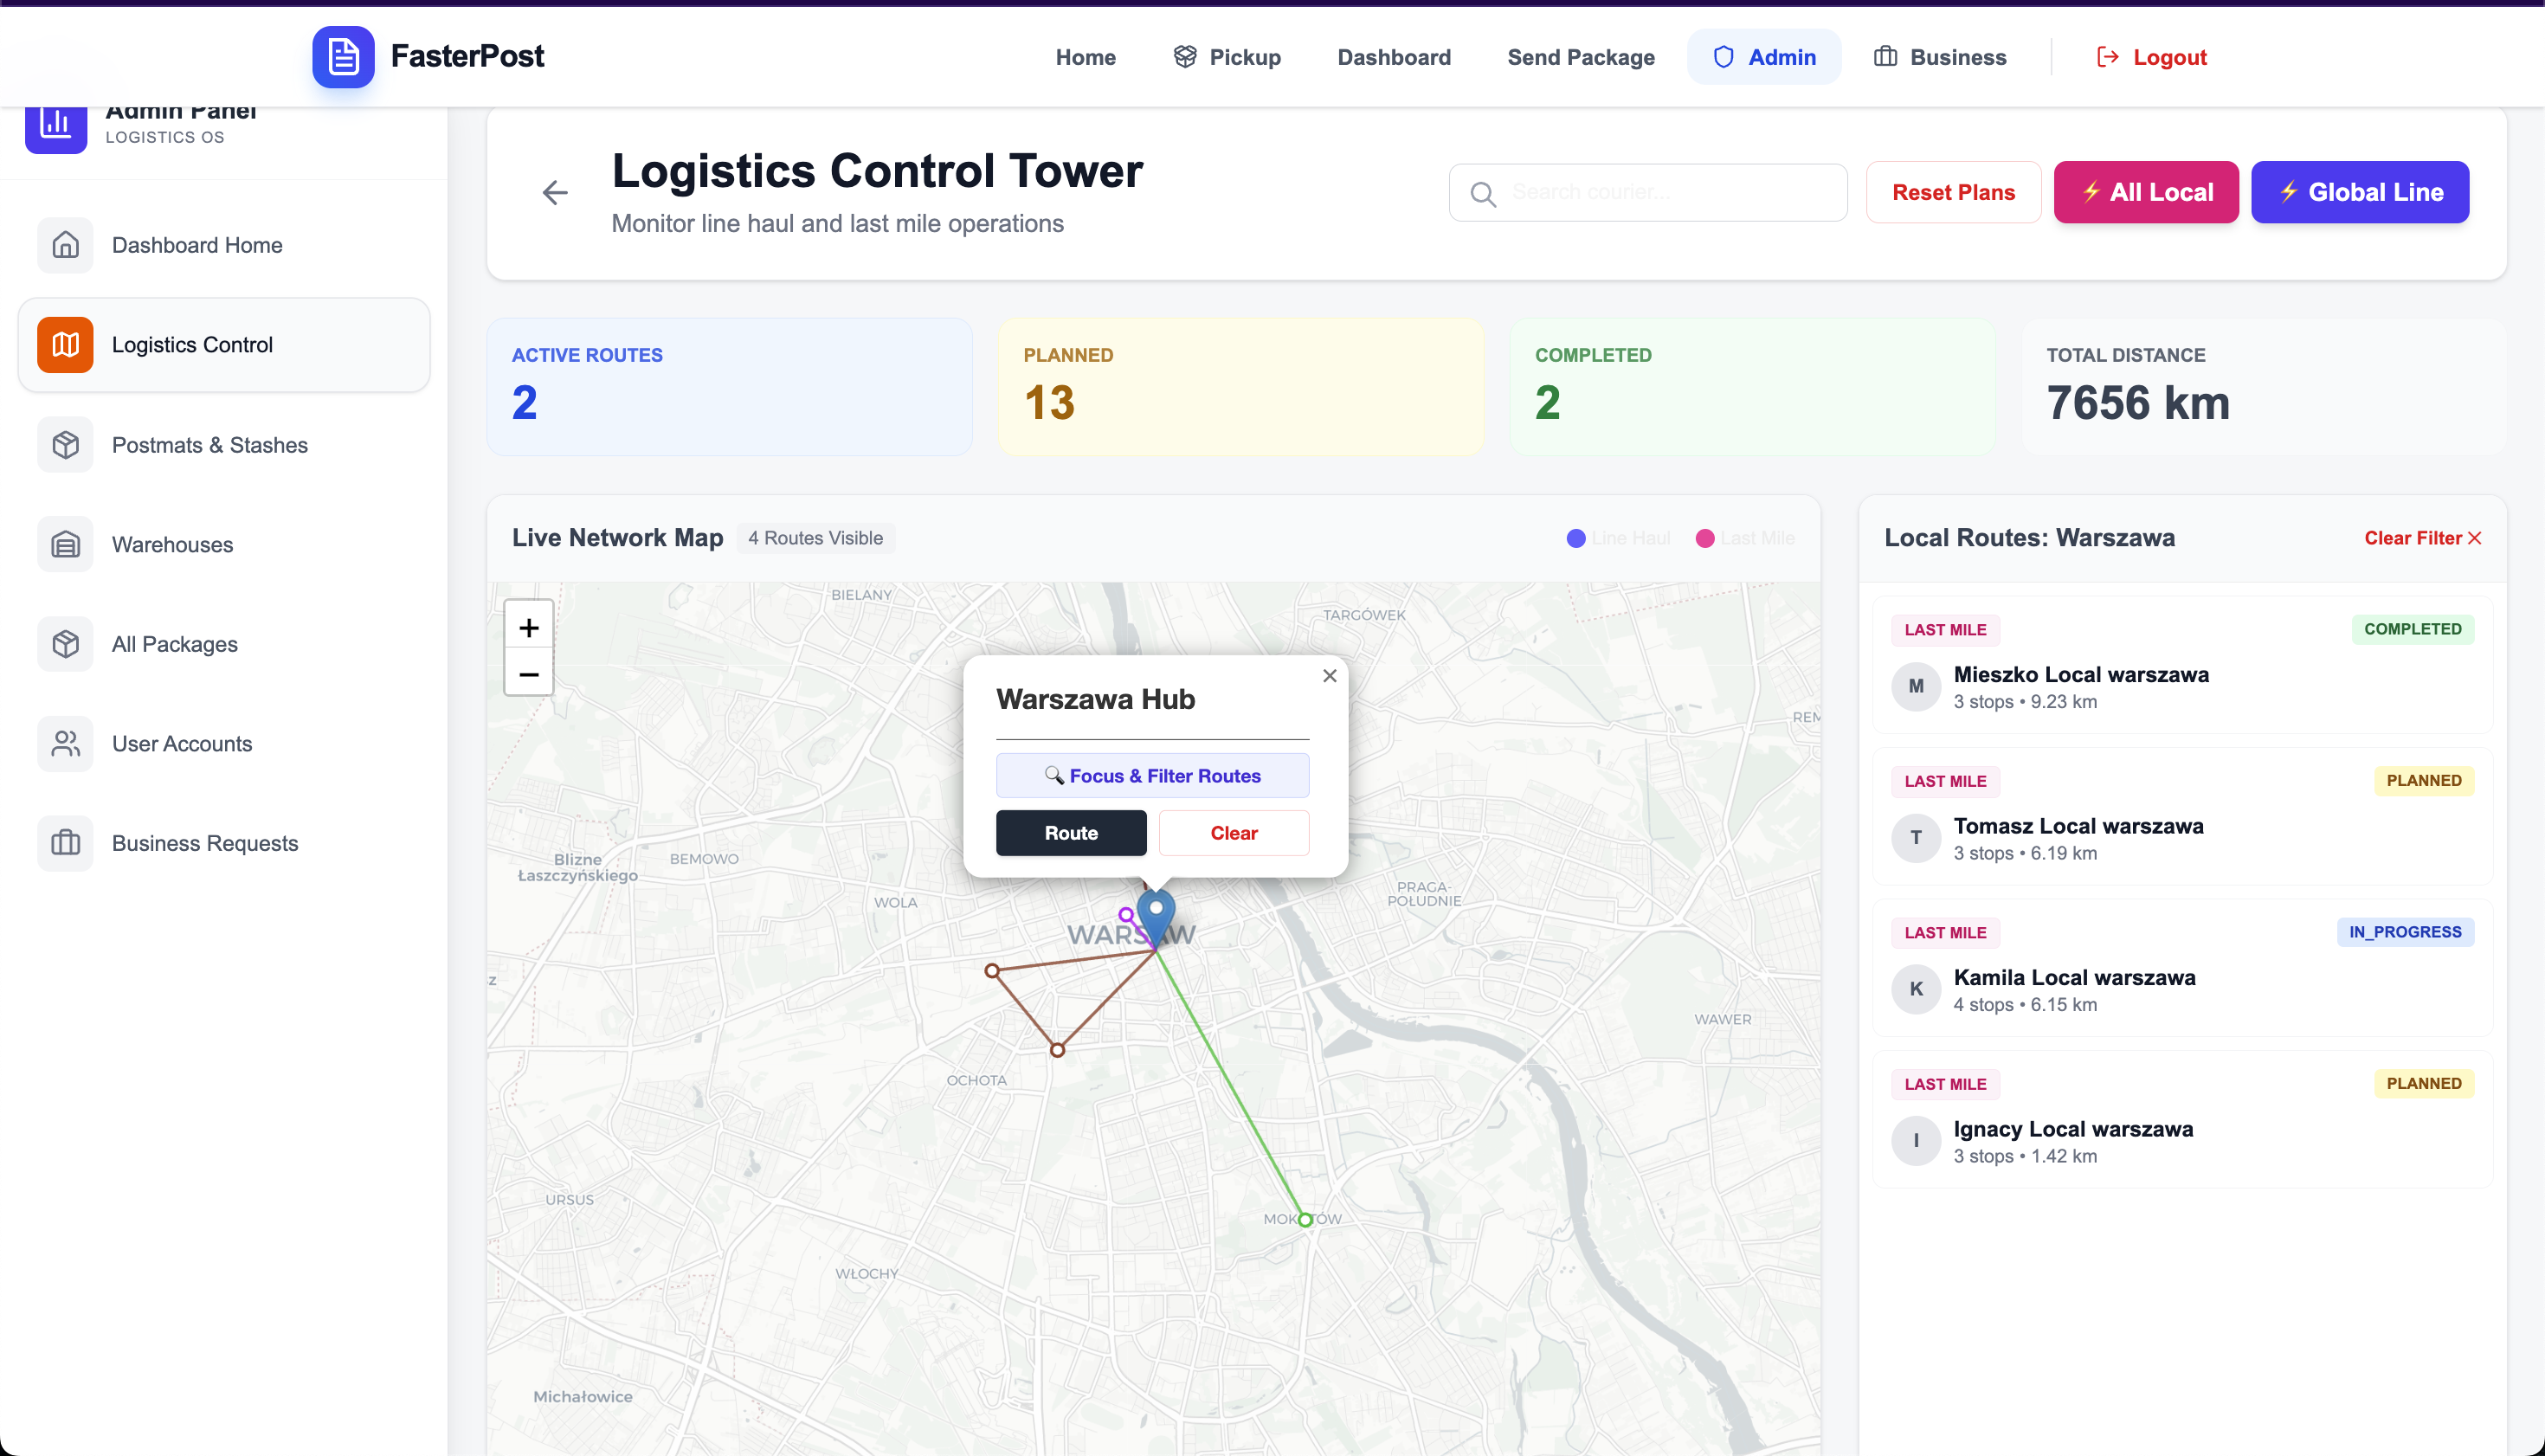
\includegraphics[width=0.7\textwidth]{../screenshots/13_isi_logistic_control_warsaw.png}
    \caption{Moduł kontroli logistycznej z wizualizacją mapy.}
\end{figure}

\begin{figure}[H]
    \centering
    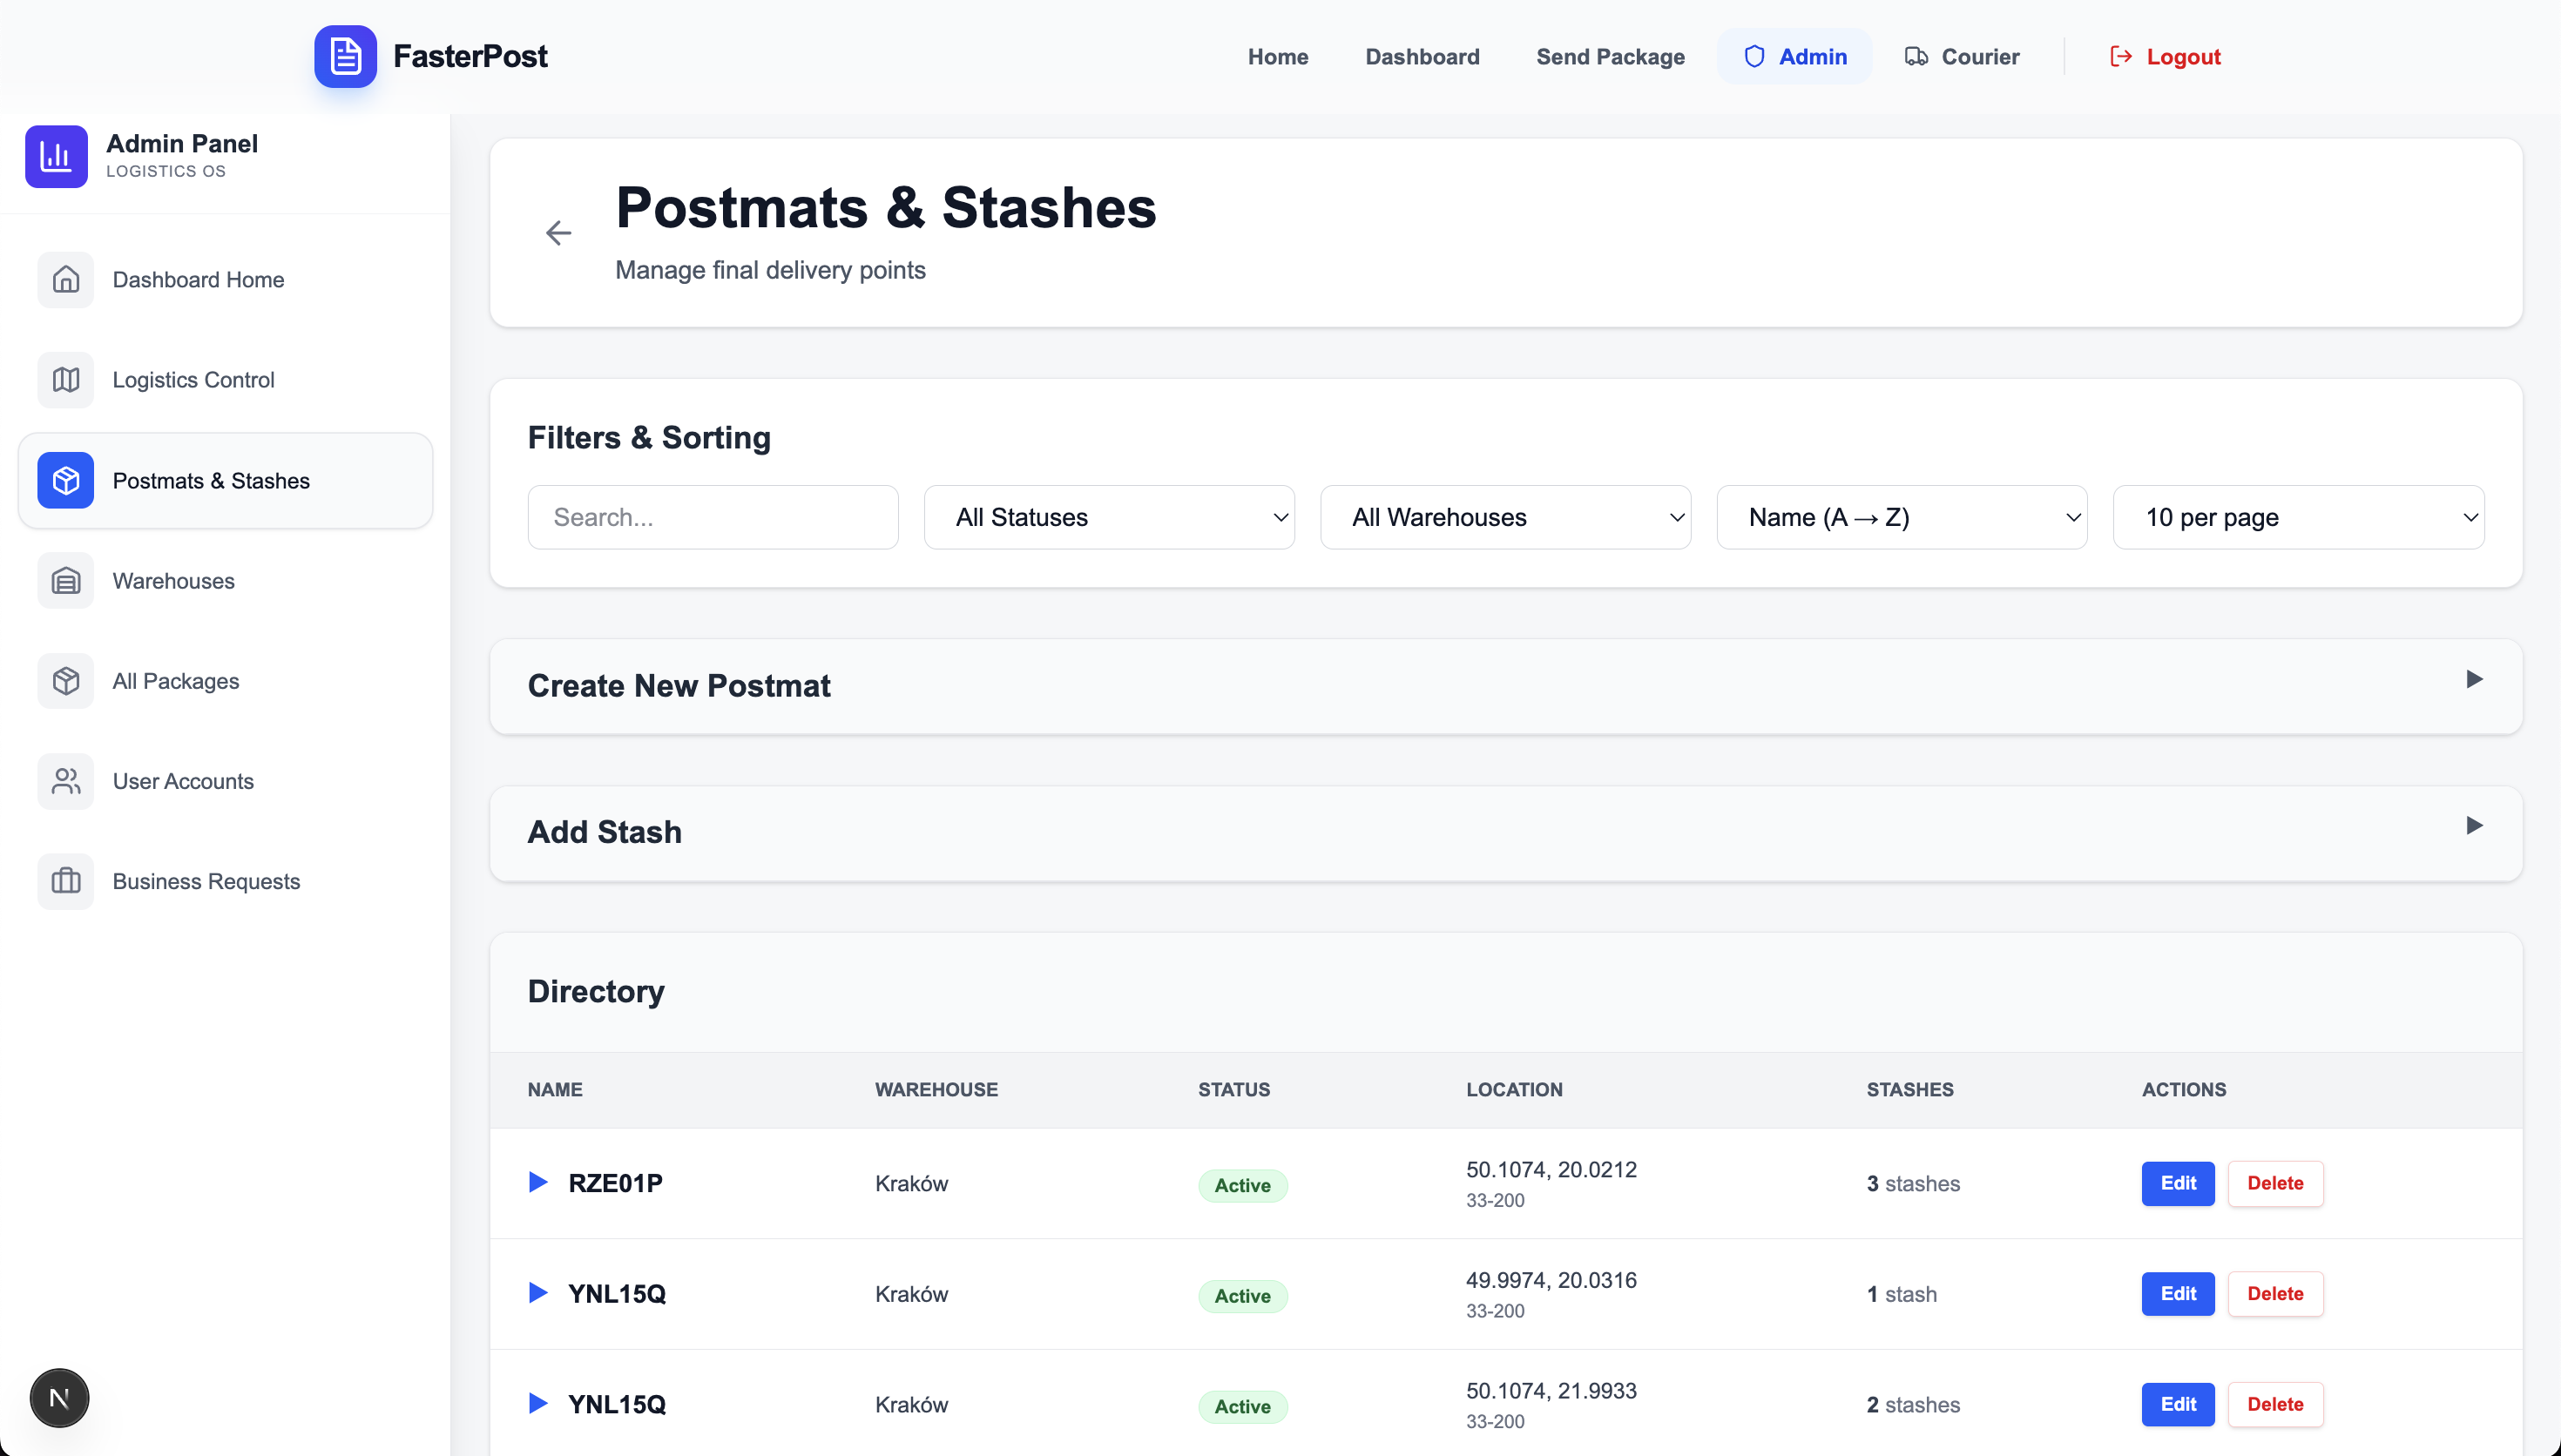
\includegraphics[width=0.45\textwidth]{../screenshots/12_admin_postmats_and_stashes.png}
    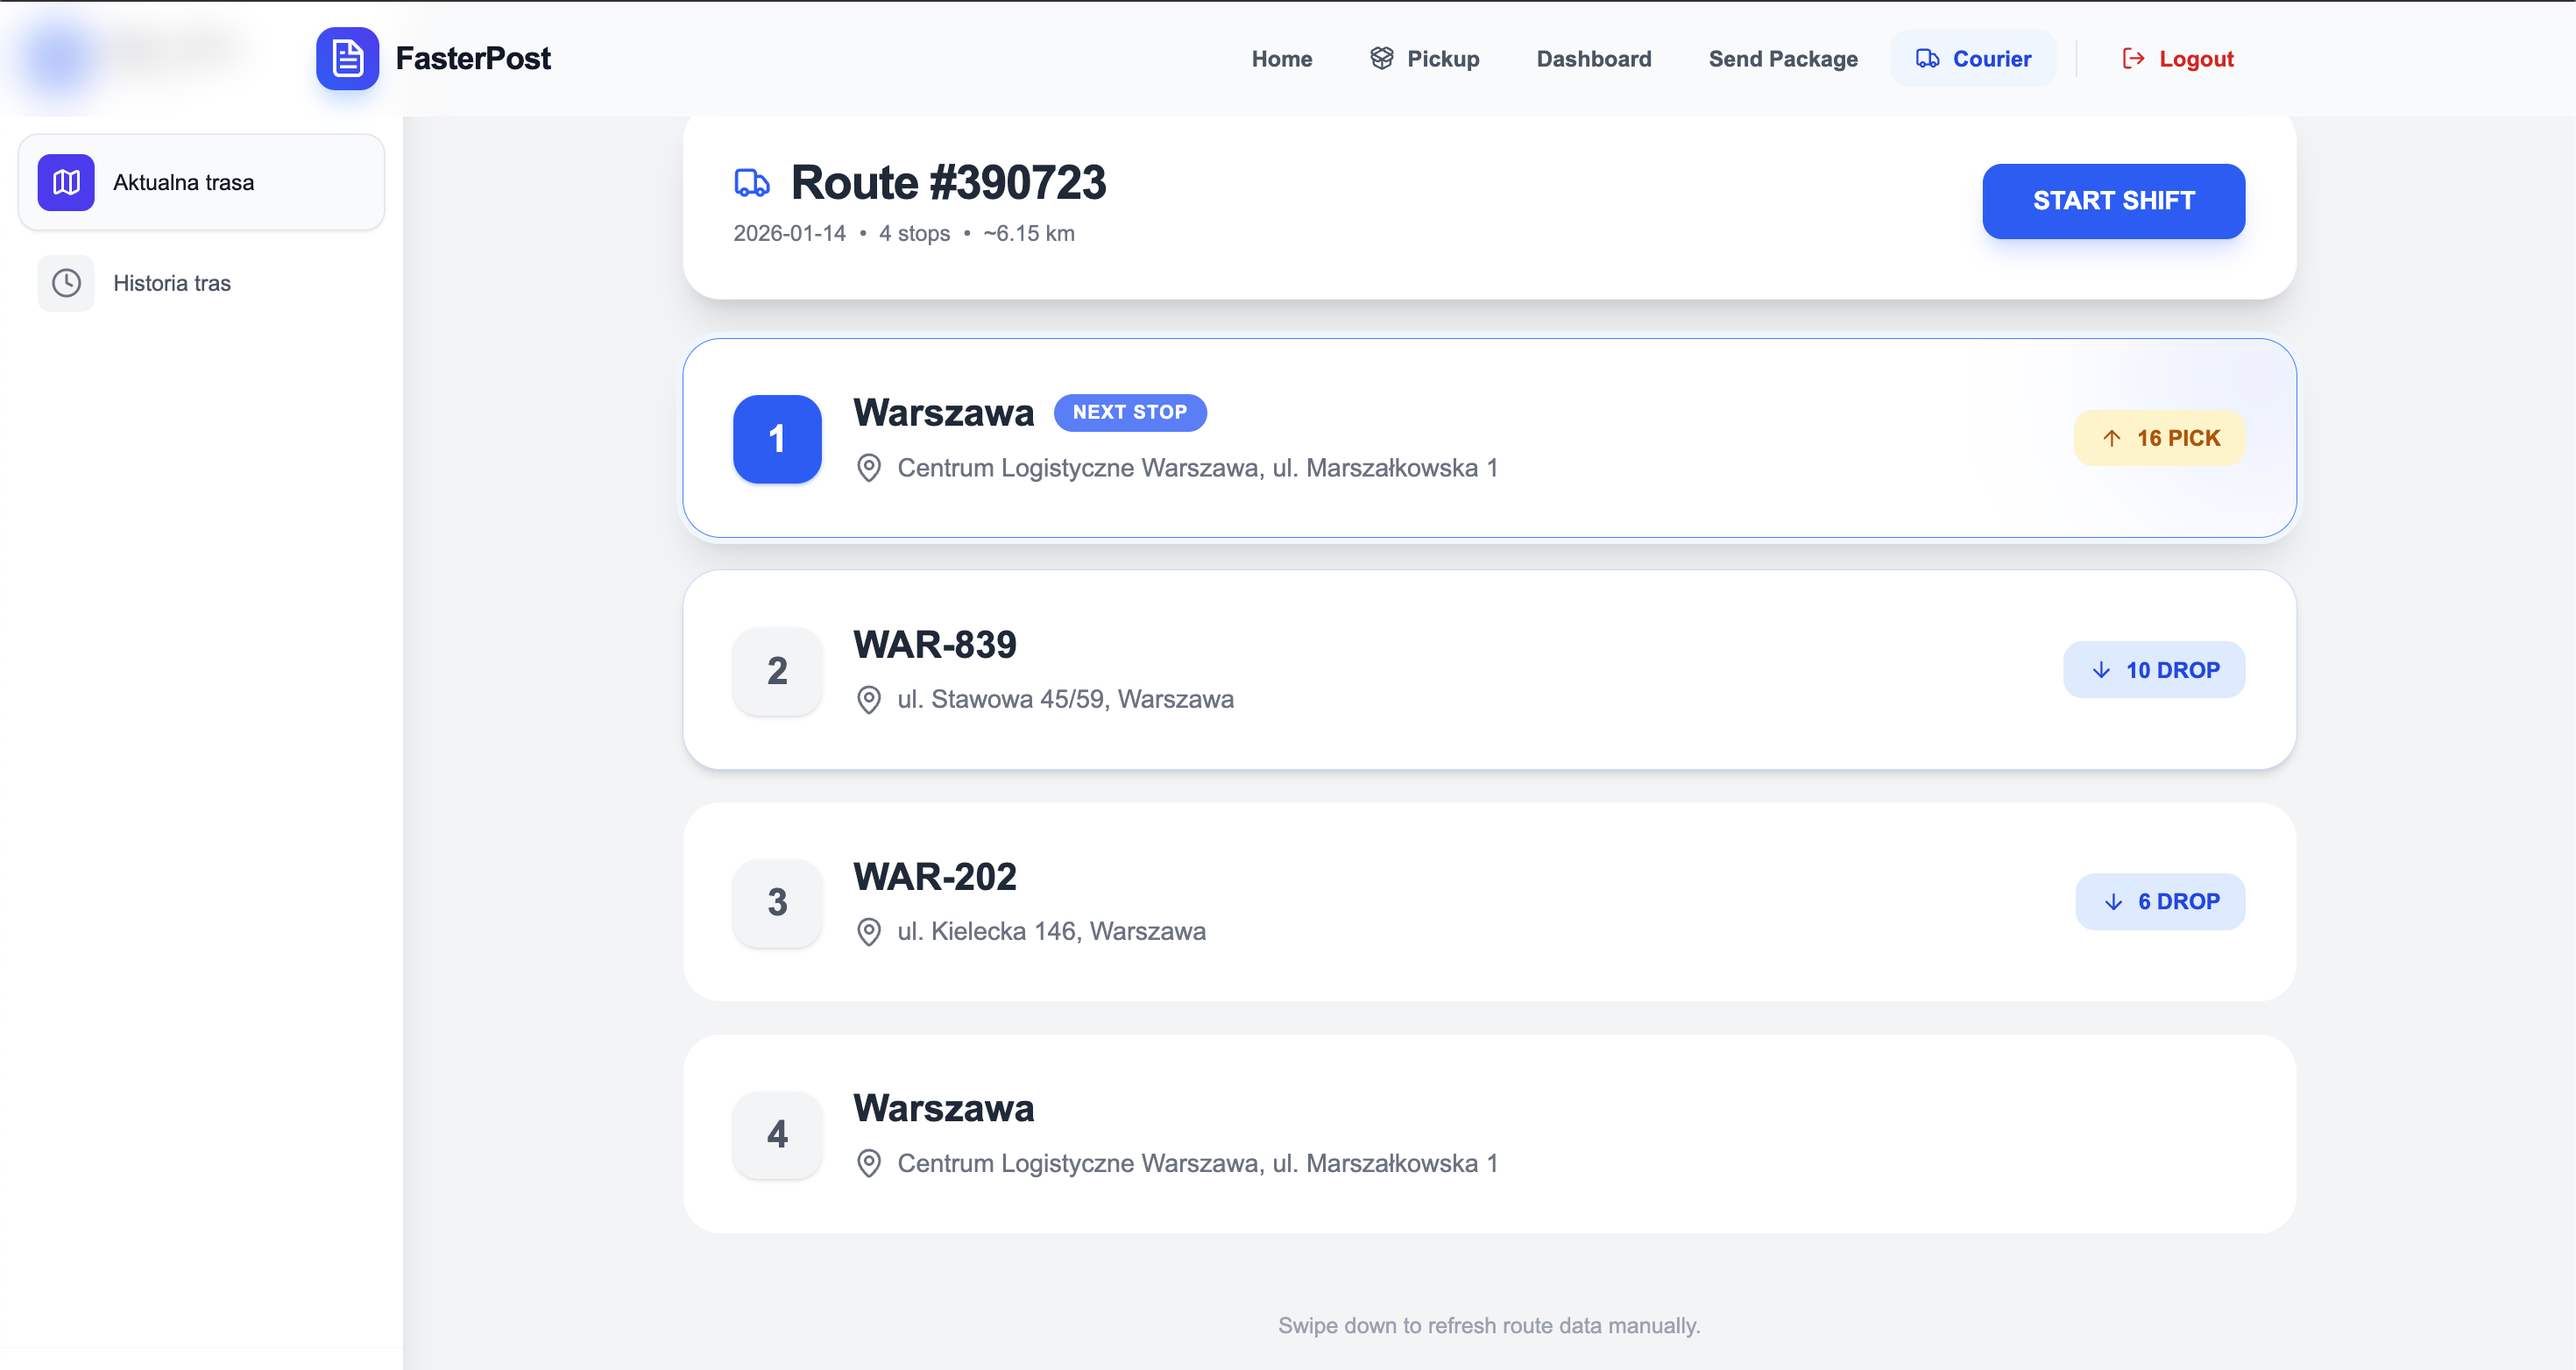
\includegraphics[width=0.45\textwidth]{../screenshots/13_isi_localcourier_panel.png}
    \caption{Zarządzanie automatami paczkowymi oraz panel kuriera lokalnego.}
\end{figure}

\section{Elementy pomocnicze}
W celu poprawy użyteczności zastosowano wzorce informacyjne, takie jak FAQ (Accordion) oraz systemy pomocy.

\begin{figure}[H]
    \centering
    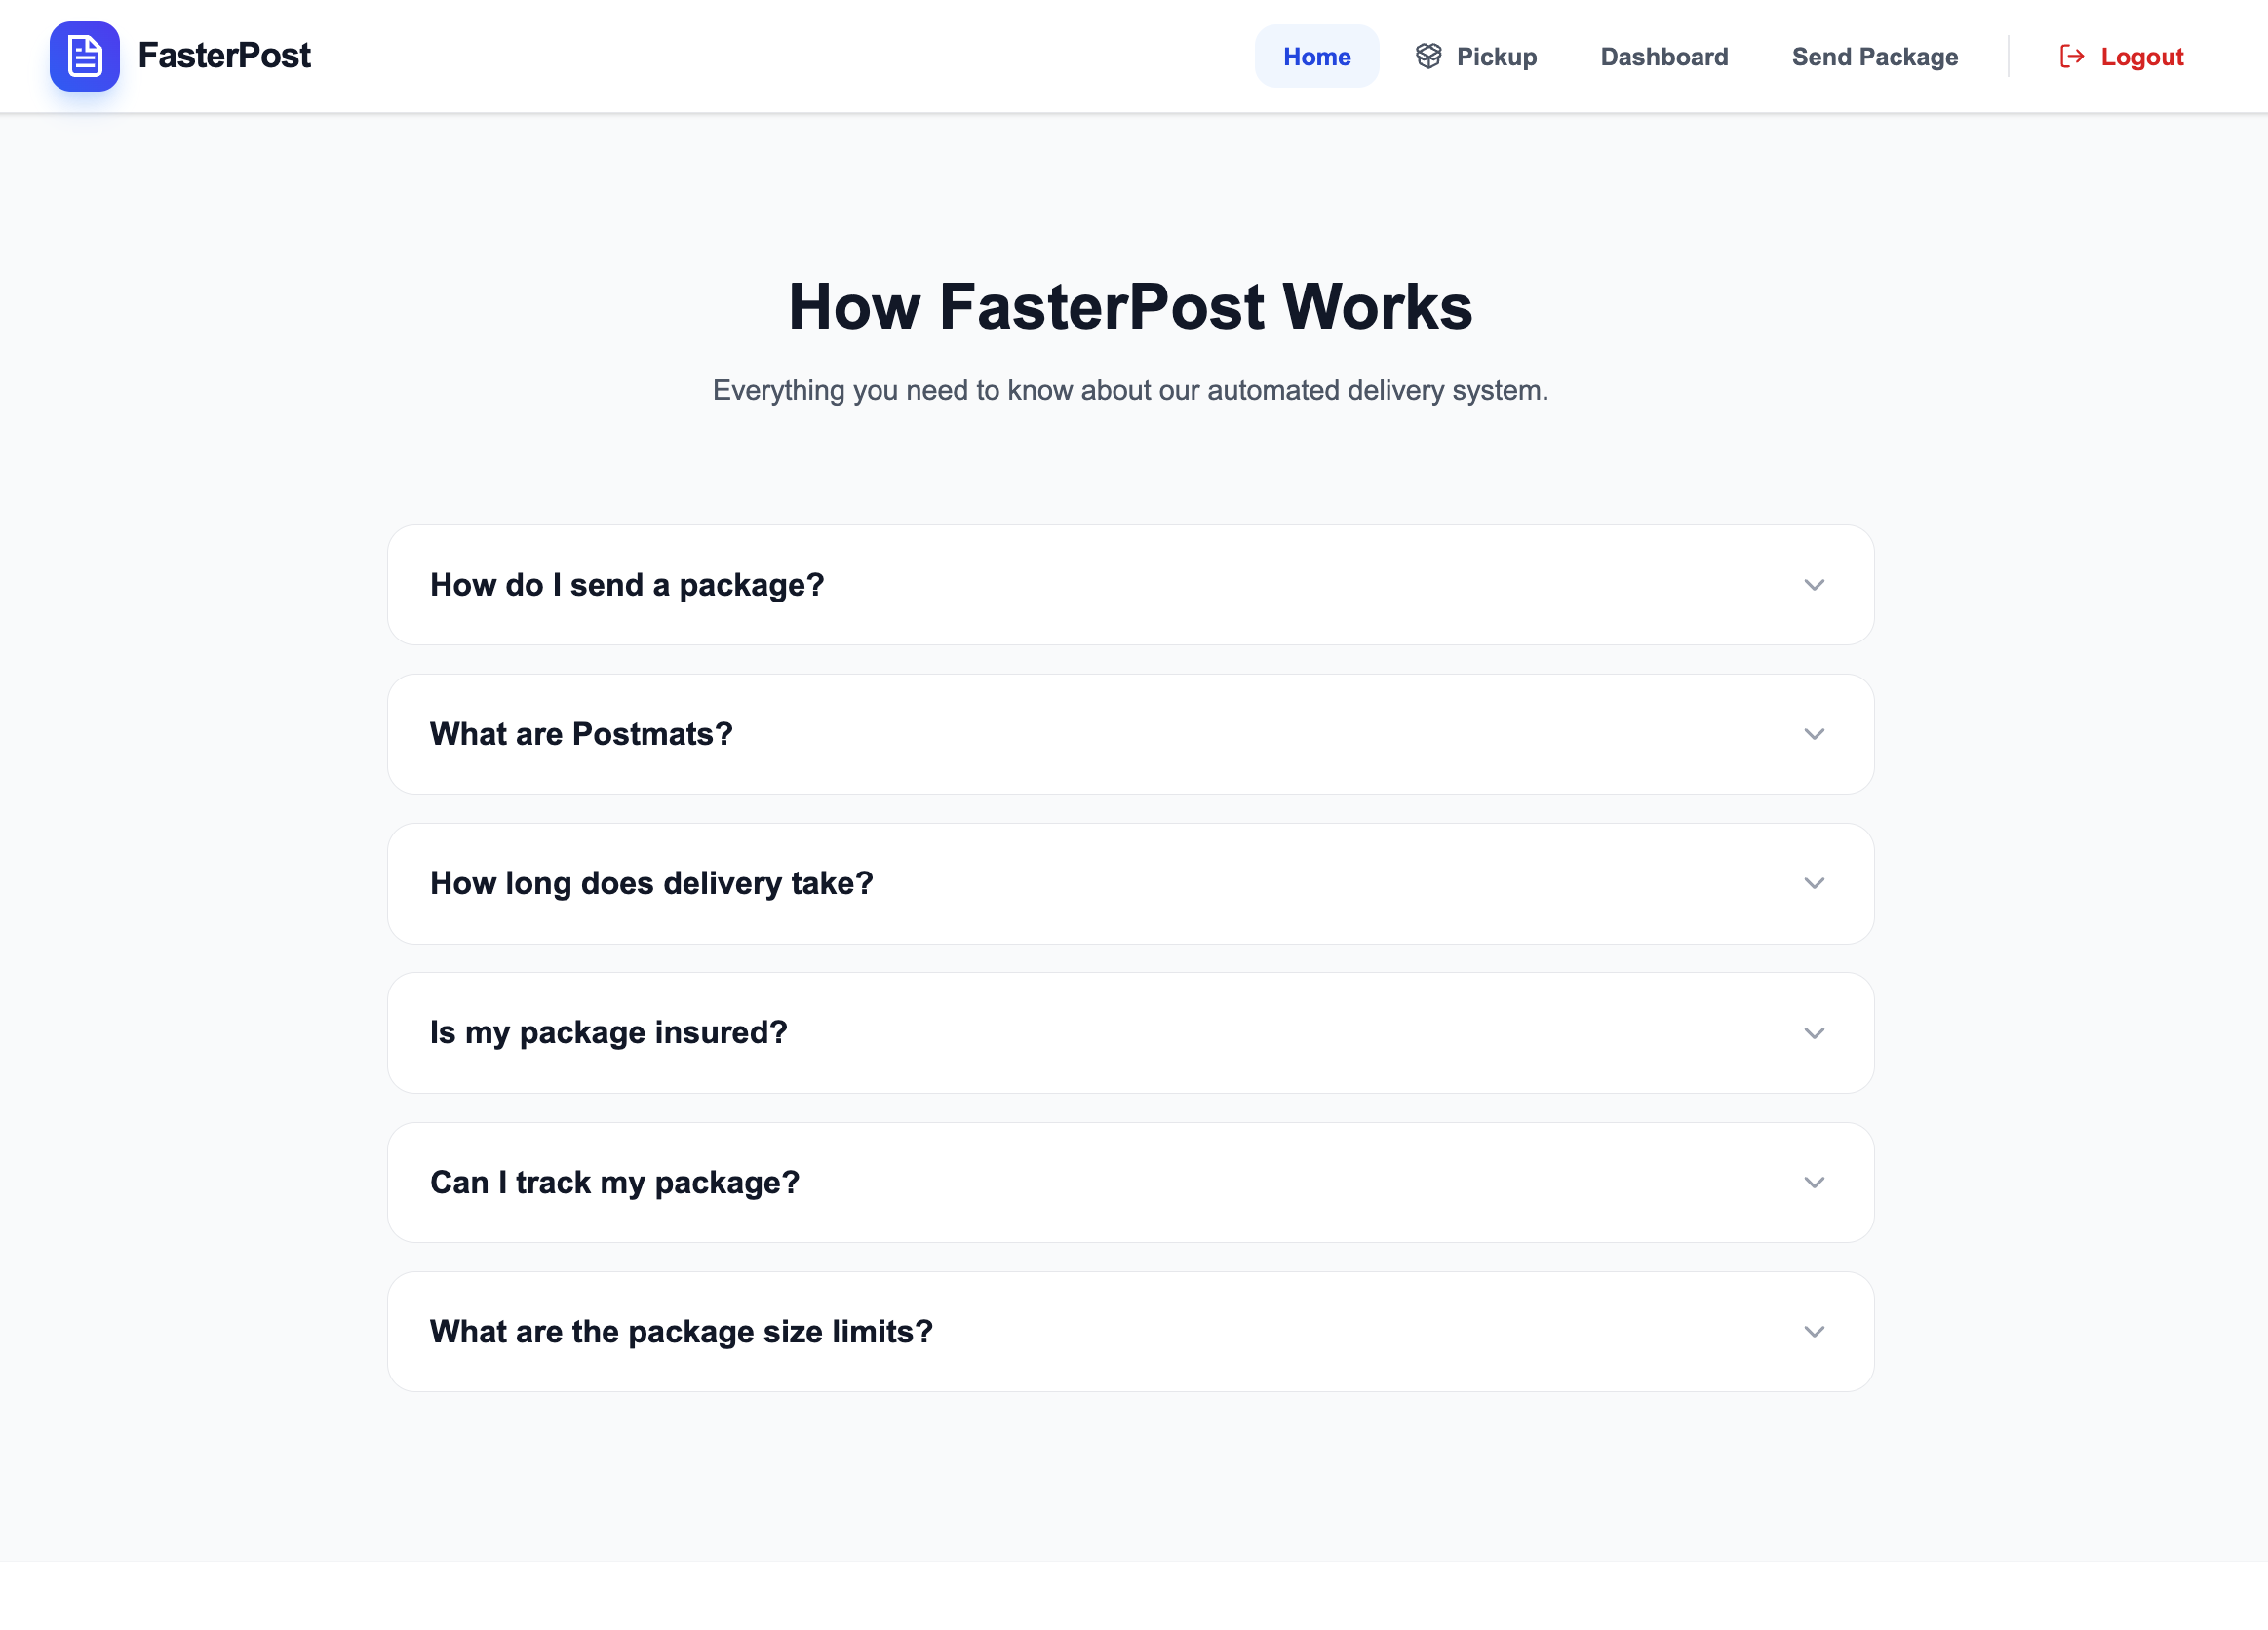
\includegraphics[width=0.6\textwidth]{../screenshots/5_faq.png}
    \caption{Sekcja FAQ wykorzystująca wzorzec Accordion.}
\end{figure}

\section{Podsumowanie projektowe}
Zaprojektowany interfejs spełnia zasady prostoty, minimalizmu oraz responsywności. Wykorzystanie sprawdzonych wzorców (Side Navigation, Cards, Modal Windows) zapewnia intuicyjność środowiska dla użytkownika końcowego, niezależnie od pełnionej roli w systemie (klient, biznes, kurier czy administrator).